\documentclass[]{article}
\usepackage{lmodern}
\usepackage{amssymb,amsmath}
\usepackage{ifxetex,ifluatex}
\usepackage{fixltx2e} % provides \textsubscript
\ifnum 0\ifxetex 1\fi\ifluatex 1\fi=0 % if pdftex
  \usepackage[T1]{fontenc}
  \usepackage[utf8]{inputenc}
\else % if luatex or xelatex
  \ifxetex
    \usepackage{mathspec}
  \else
    \usepackage{fontspec}
  \fi
  \defaultfontfeatures{Ligatures=TeX,Scale=MatchLowercase}
\fi
% use upquote if available, for straight quotes in verbatim environments
\IfFileExists{upquote.sty}{\usepackage{upquote}}{}
% use microtype if available
\IfFileExists{microtype.sty}{%
\usepackage{microtype}
\UseMicrotypeSet[protrusion]{basicmath} % disable protrusion for tt fonts
}{}
\usepackage[margin=1in]{geometry}
\usepackage{hyperref}
\hypersetup{unicode=true,
            pdftitle={Final Report: Identification of SSTs},
            pdfauthor={Elias Benjamin Farr, Lennart Linke, Lisa Marie Milchsack, Salome Steinke},
            pdfborder={0 0 0},
            breaklinks=true}
\urlstyle{same}  % don't use monospace font for urls
\usepackage{color}
\usepackage{fancyvrb}
\newcommand{\VerbBar}{|}
\newcommand{\VERB}{\Verb[commandchars=\\\{\}]}
\DefineVerbatimEnvironment{Highlighting}{Verbatim}{commandchars=\\\{\}}
% Add ',fontsize=\small' for more characters per line
\usepackage{framed}
\definecolor{shadecolor}{RGB}{248,248,248}
\newenvironment{Shaded}{\begin{snugshade}}{\end{snugshade}}
\newcommand{\AlertTok}[1]{\textcolor[rgb]{0.94,0.16,0.16}{#1}}
\newcommand{\AnnotationTok}[1]{\textcolor[rgb]{0.56,0.35,0.01}{\textbf{\textit{#1}}}}
\newcommand{\AttributeTok}[1]{\textcolor[rgb]{0.77,0.63,0.00}{#1}}
\newcommand{\BaseNTok}[1]{\textcolor[rgb]{0.00,0.00,0.81}{#1}}
\newcommand{\BuiltInTok}[1]{#1}
\newcommand{\CharTok}[1]{\textcolor[rgb]{0.31,0.60,0.02}{#1}}
\newcommand{\CommentTok}[1]{\textcolor[rgb]{0.56,0.35,0.01}{\textit{#1}}}
\newcommand{\CommentVarTok}[1]{\textcolor[rgb]{0.56,0.35,0.01}{\textbf{\textit{#1}}}}
\newcommand{\ConstantTok}[1]{\textcolor[rgb]{0.00,0.00,0.00}{#1}}
\newcommand{\ControlFlowTok}[1]{\textcolor[rgb]{0.13,0.29,0.53}{\textbf{#1}}}
\newcommand{\DataTypeTok}[1]{\textcolor[rgb]{0.13,0.29,0.53}{#1}}
\newcommand{\DecValTok}[1]{\textcolor[rgb]{0.00,0.00,0.81}{#1}}
\newcommand{\DocumentationTok}[1]{\textcolor[rgb]{0.56,0.35,0.01}{\textbf{\textit{#1}}}}
\newcommand{\ErrorTok}[1]{\textcolor[rgb]{0.64,0.00,0.00}{\textbf{#1}}}
\newcommand{\ExtensionTok}[1]{#1}
\newcommand{\FloatTok}[1]{\textcolor[rgb]{0.00,0.00,0.81}{#1}}
\newcommand{\FunctionTok}[1]{\textcolor[rgb]{0.00,0.00,0.00}{#1}}
\newcommand{\ImportTok}[1]{#1}
\newcommand{\InformationTok}[1]{\textcolor[rgb]{0.56,0.35,0.01}{\textbf{\textit{#1}}}}
\newcommand{\KeywordTok}[1]{\textcolor[rgb]{0.13,0.29,0.53}{\textbf{#1}}}
\newcommand{\NormalTok}[1]{#1}
\newcommand{\OperatorTok}[1]{\textcolor[rgb]{0.81,0.36,0.00}{\textbf{#1}}}
\newcommand{\OtherTok}[1]{\textcolor[rgb]{0.56,0.35,0.01}{#1}}
\newcommand{\PreprocessorTok}[1]{\textcolor[rgb]{0.56,0.35,0.01}{\textit{#1}}}
\newcommand{\RegionMarkerTok}[1]{#1}
\newcommand{\SpecialCharTok}[1]{\textcolor[rgb]{0.00,0.00,0.00}{#1}}
\newcommand{\SpecialStringTok}[1]{\textcolor[rgb]{0.31,0.60,0.02}{#1}}
\newcommand{\StringTok}[1]{\textcolor[rgb]{0.31,0.60,0.02}{#1}}
\newcommand{\VariableTok}[1]{\textcolor[rgb]{0.00,0.00,0.00}{#1}}
\newcommand{\VerbatimStringTok}[1]{\textcolor[rgb]{0.31,0.60,0.02}{#1}}
\newcommand{\WarningTok}[1]{\textcolor[rgb]{0.56,0.35,0.01}{\textbf{\textit{#1}}}}
\usepackage{longtable,booktabs}
\usepackage{graphicx,grffile}
\makeatletter
\def\maxwidth{\ifdim\Gin@nat@width>\linewidth\linewidth\else\Gin@nat@width\fi}
\def\maxheight{\ifdim\Gin@nat@height>\textheight\textheight\else\Gin@nat@height\fi}
\makeatother
% Scale images if necessary, so that they will not overflow the page
% margins by default, and it is still possible to overwrite the defaults
% using explicit options in \includegraphics[width, height, ...]{}
\setkeys{Gin}{width=\maxwidth,height=\maxheight,keepaspectratio}
\IfFileExists{parskip.sty}{%
\usepackage{parskip}
}{% else
\setlength{\parindent}{0pt}
\setlength{\parskip}{6pt plus 2pt minus 1pt}
}
\setlength{\emergencystretch}{3em}  % prevent overfull lines
\providecommand{\tightlist}{%
  \setlength{\itemsep}{0pt}\setlength{\parskip}{0pt}}
\setcounter{secnumdepth}{0}
% Redefines (sub)paragraphs to behave more like sections
\ifx\paragraph\undefined\else
\let\oldparagraph\paragraph
\renewcommand{\paragraph}[1]{\oldparagraph{#1}\mbox{}}
\fi
\ifx\subparagraph\undefined\else
\let\oldsubparagraph\subparagraph
\renewcommand{\subparagraph}[1]{\oldsubparagraph{#1}\mbox{}}
\fi

%%% Use protect on footnotes to avoid problems with footnotes in titles
\let\rmarkdownfootnote\footnote%
\def\footnote{\protect\rmarkdownfootnote}

%%% Change title format to be more compact
\usepackage{titling}

% Create subtitle command for use in maketitle
\providecommand{\subtitle}[1]{
  \posttitle{
    \begin{center}\large#1\end{center}
    }
}

\setlength{\droptitle}{-2em}

  \title{Final Report: Identification of SSTs}
    \pretitle{\vspace{\droptitle}\centering\huge}
  \posttitle{\par}
    \author{Elias Benjamin Farr, Lennart Linke, Lisa Marie Milchsack, Salome Steinke}
    \preauthor{\centering\large\emph}
  \postauthor{\par}
      \predate{\centering\large\emph}
  \postdate{\par}
    \date{17. Juli 2019}


\begin{document}
\maketitle

{
\setcounter{tocdepth}{2}
\tableofcontents
}
\hypertarget{introduction}{%
\section{Introduction}\label{introduction}}

\hypertarget{breast-cancer-a-challenging-disease}{%
\subsection{Breast Cancer: a challenging
disease}\label{breast-cancer-a-challenging-disease}}

\begin{quote}
``The heterogeneity of breast cancers makes them both a fascinating and
challenging solid tumor to diagnose and treat.''

Raj Kumar (2016) in A novel therapeutic target for triple negative
breast cancer
\end{quote}

Breast cancer (BC) is currently known as one of the most prevalent and
deathly malignant tumor types, resulting in more than 600,000 deaths
worldwide in 2017 (GBD 2017). While in Germany 70,000 new cases are
reported annually (Barnes, Kraywinkel et al.~2016), breast cancer makes
up \textasciitilde30\% of all reported cases of tumor diseases
(Robert-Koch-Institut 2017). Over the past 27 years the prevalence of
this tumor surged by one sixth in percentage of world population,
calling for accelerated research on possible therapy options. While in
the past decades breast cancer therapy has already evolved, reducing the
age standardized death rate by one third, from 15.10 to only 10.00 in
western europe (GBD 2017), the necessity to find effective prevention
methods remains (Sledge et al.~2014). A promising method is an
computerbased approach taking identifying genetic interactions which can
be exploited therapeutically. This stratetgy is also pursued by the
project at hand.

\hypertarget{driver-mutations-the-driving-force-in-tumorigenesis}{%
\subsection{Driver Mutations: the driving force in
tumorigenesis}\label{driver-mutations-the-driving-force-in-tumorigenesis}}

Driver mutations (DV) are the key promoters of tumorigenesis leading to
new functions and cell states of affected tissues (Stratton, 2009).
Thus, the acquisition of driver mutations is essential for tumour
initiation, transformation as well as progression and metastasis
(Hanahan, 2000). According to Bert Vogelstein three mutations in genes
displaying a crucial function in cell proliferation, DNA integrity and
cellular motility are enough to drive a normal cell into aberrant growth
and malignancy:

\begin{quote}
``Focusing on driver-gene mutations and the pathways they control has
rendered complex cancer-genome landscapes intelligible. In solid tumors
of adults, alterations in as few as three driver genes appear to suffice
for a cell to evolve into an advanced cancer.''

Bert Vogelstein in The Path to Cancer - Three Strikes and You're Out
\end{quote}

These DVs comprise both gain-of-function mutations in (proto-)oncogenes
which usually promote cell proliferation and loss-of-function mutations
in tumour suppressor genes which usually decelerate the cell cycle as
well as genes involved in DNA repair and proofreading (Anderson, 1992;
Lee, 2010). Thereby, the cell acquires indispensable properties in
tumorigenesis such as immortality, continous proliferation, immune and
apoptosis resistance and the ability to promote angiogenesis (Hanahan,
2000). Examples for prominent oncogenes are k-ras and b-raf, both
encoding kinases, regulating a complex network of proteins involved in
cellular growth when bound to ATP or GTP, respectively. On the other
hand, the most illustrious tumour suppressor gene is p53 whose
physiological role is to induce cell senescence and apoptosis in case of
DNA damage, a condition often encountered in cancer cells (Tsilimigras,
2018; Lee, 2010).

Due to their essential role in tumour progression DVs are predisposed
targets in novel approaches in cancer therapy (Nussinov, 2019). For
instance an antibody against HER2 (trastuzumab), which is an oncogene
promoting cell growth while inhibiting apotosis, launched in 1998 was
proven to reduce the recurrence rate by 50\% and mortality by 30\%
(Maximiano, 2016). However, targeting genes or gene products involved in
vital cellular processes remains a major challenge as healthy cells
expressing the same genes are often affected as well (Lacouture, 2018).
As therapies tailored to the molecular phenotype of the tumour achieved
greater successes than conventional strategies, such as chemotherapy and
irradiation, scientists now focus on identifying other molecular targets
with a negligible effect on healthy tissues.

\hypertarget{second-site-targets-secret-co-operators-in-tumorigenesis}{%
\subsection{Second-site targets: secret co-operators in
tumorigenesis}\label{second-site-targets-secret-co-operators-in-tumorigenesis}}

Driver mutations are not the only genetic factors involved in cancer
development. Moreover, tumorigenesis derives from a complex genetic
programme comprising several minor and major alterations in gene
expression patterns as well as protein regulation. As these factors act
synergistically in promoting tumour growth disturbing their interaction
might provide another method of inhibiting cancer proliferation
(Ashworth, 2011).

The considered factors supporting the effect of driver mutations are
often referred to as second-site targets (SSTs, also called
``landscapers'') as they do not necessarily confer a growth advantage to
the tumour when mutated alone but by genetic interaction with other
mutations. Thus, SSTs constitute promising targets in cancer therapy as
they are meant to have a less significant effect on the viability of
healthy cells because they do not display central regulatory functions
(Ashworth, 2011). However, identification of these secret co-operators
demands the analysis of several parameters reflecting their relevance
and function in proliferation such as RNAseq data, data from gene
knockouts and mutational analyses (Rauscher, 2018; Benstead-Hume, 2017;
Magen, 2018).

\begin{figure}

{\centering 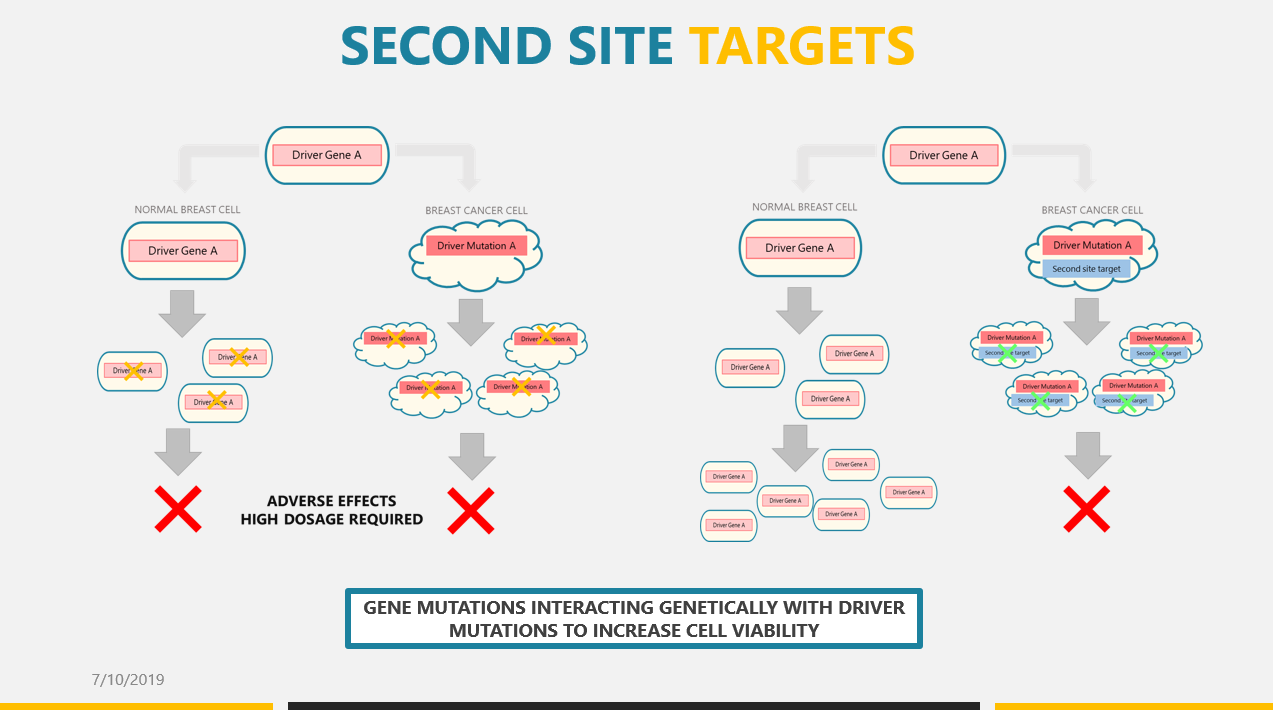
\includegraphics[width=1\linewidth]{Concept_of_SSTs} 

}

\caption{Concept of SSTs}\label{fig:SSTs}
\end{figure}

\hypertarget{project-outline}{%
\section{Project outline}\label{project-outline}}

The aim of this project is to answer the central question:

\begin{quote}
Which \textbf{second-site targets} interact genetically with
\textbf{driver mutations} to promote cell viability and proliferation in
breast cell cancers?
\end{quote}

To begin with possible driver mutations from literature research were
selected based on the following three characteristics:

\begin{enumerate}
\def\labelenumi{\arabic{enumi}.}
\tightlist
\item
  overexpressed in breast cancer
\item
  observed in a relevant percentage of clinical cases
\item
  part of processes/pathways of tumorgenesis
\end{enumerate}

Finally, we selected:

\begin{longtable}[]{@{}llll@{}}
\toprule
\begin{minipage}[b]{0.07\columnwidth}\raggedright
Gene Name\strut
\end{minipage} & \begin{minipage}[b]{0.14\columnwidth}\raggedright
Overexpression rate\strut
\end{minipage} & \begin{minipage}[b]{0.27\columnwidth}\raggedright
Role in Tumorgenesis\strut
\end{minipage} & \begin{minipage}[b]{0.41\columnwidth}\raggedright
Sources\strut
\end{minipage}\tabularnewline
\midrule
\endhead
\begin{minipage}[t]{0.07\columnwidth}\raggedright
CCND\strut
\end{minipage} & \begin{minipage}[t]{0.14\columnwidth}\raggedright
\textasciitilde{} 50\%\strut
\end{minipage} & \begin{minipage}[t]{0.27\columnwidth}\raggedright
Cell cycle regulator\strut
\end{minipage} & \begin{minipage}[t]{0.41\columnwidth}\raggedright
(Arnold and Papanikolaou 2005)\strut
\end{minipage}\tabularnewline
\begin{minipage}[t]{0.07\columnwidth}\raggedright
ERBB2\strut
\end{minipage} & \begin{minipage}[t]{0.14\columnwidth}\raggedright
\textasciitilde{} 30\%\strut
\end{minipage} & \begin{minipage}[t]{0.27\columnwidth}\raggedright
Encodes endothelial growth factor\strut
\end{minipage} & \begin{minipage}[t]{0.41\columnwidth}\raggedright
(Slamon, Godolphin et al.~1989)\strut
\end{minipage}\tabularnewline
\begin{minipage}[t]{0.07\columnwidth}\raggedright
MYC\strut
\end{minipage} & \begin{minipage}[t]{0.14\columnwidth}\raggedright
\textasciitilde{} 30 - 50\%\strut
\end{minipage} & \begin{minipage}[t]{0.27\columnwidth}\raggedright
Cell cycle and apoptosis regulator\strut
\end{minipage} & \begin{minipage}[t]{0.41\columnwidth}\raggedright
(Gabay, Li et al.~, Xu, Chen et al.~2010)\strut
\end{minipage}\tabularnewline
\begin{minipage}[t]{0.07\columnwidth}\raggedright
PARP10\strut
\end{minipage} & \begin{minipage}[t]{0.14\columnwidth}\raggedright
\textasciitilde{} 45\%\strut
\end{minipage} & \begin{minipage}[t]{0.27\columnwidth}\raggedright
Regulates differentiation/proliferation\strut
\end{minipage} & \begin{minipage}[t]{0.41\columnwidth}\raggedright
(Siraj, Pratheeshkumar et al.~2018)\strut
\end{minipage}\tabularnewline
\begin{minipage}[t]{0.07\columnwidth}\raggedright
PIK3CA\strut
\end{minipage} & \begin{minipage}[t]{0.14\columnwidth}\raggedright
\textasciitilde{} 30 - 48\%\strut
\end{minipage} & \begin{minipage}[t]{0.27\columnwidth}\raggedright
Interaction with AKT and mTOR pathway\strut
\end{minipage} & \begin{minipage}[t]{0.41\columnwidth}\raggedright
(Aleskandarany, Rakha et al.~2010, Shimoi, Hamada et al.2018)\strut
\end{minipage}\tabularnewline
\bottomrule
\end{longtable}

\textbackslash begin\{figure\}

\{\centering 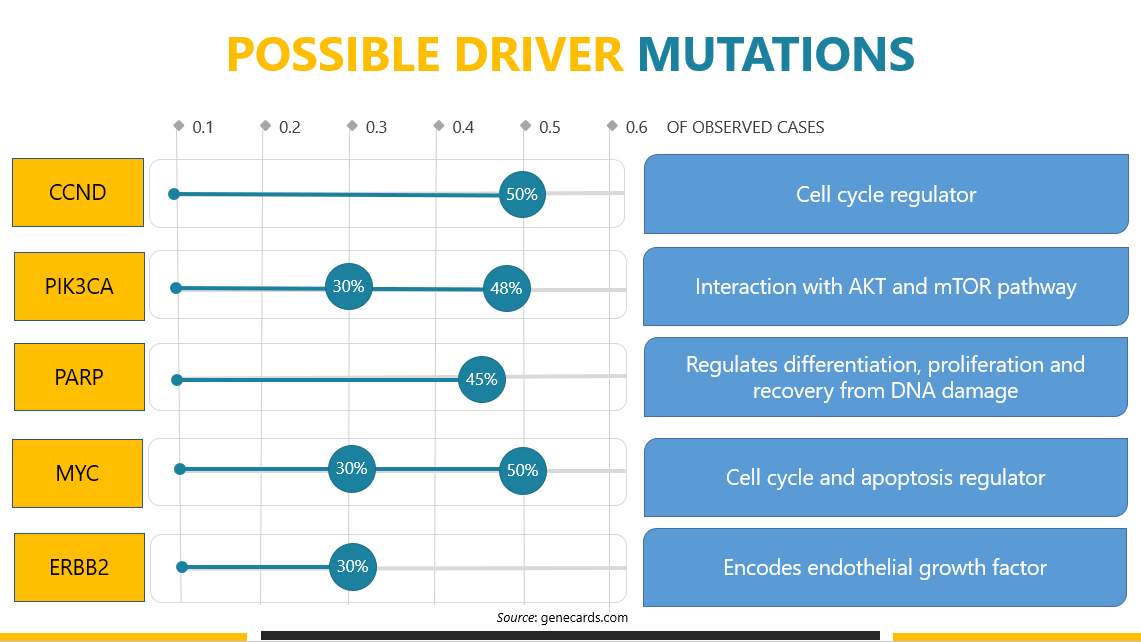
\includegraphics[width=1\linewidth]{Possible_Driver_Mutations}

\}

\textbackslash caption\{Possible\_Driver\_Mutations\}\label{fig:driver mutations}
\textbackslash end\{figure\}

In the following project the CERES and expression scores of these driver
mutations will be analysed together with those of the remaining mutated
genes to identify possible genetic interactions marking them as SSTs.

\hypertarget{methods}{%
\section{Methods}\label{methods}}

\hypertarget{data-cleanup-and-exploration}{%
\subsection{Data cleanup and
exploration}\label{data-cleanup-and-exploration}}

At the beginning of the analysis the data needs to be loaded:

\begin{Shaded}
\begin{Highlighting}[]
\CommentTok{#Setting a sys-path}
\NormalTok{root.dir =}\StringTok{ }\KeywordTok{dirname}\NormalTok{(rstudioapi}\OperatorTok{::}\KeywordTok{getSourceEditorContext}\NormalTok{()}\OperatorTok{$}\NormalTok{path)}

\CommentTok{#Importing the data}
\NormalTok{data =}\StringTok{ }\KeywordTok{readRDS}\NormalTok{(}\KeywordTok{paste0}\NormalTok{(root.dir, }\StringTok{"/DepMap19Q1_allData.RDS"}\NormalTok{)) }\CommentTok{#Read in the data }
\end{Highlighting}
\end{Shaded}

We had a look at the given data structure.

The dataset used contains six smaller datasets. Five of them are large
data frames while the sixth (mutation data) is a list of data frames.
For the extraction of this sixth variable we first separated it as a
list from the others, which was easier to handle.

\begin{Shaded}
\begin{Highlighting}[]
\CommentTok{#Extract the mutation data}
\NormalTok{mut <-}\StringTok{ }\NormalTok{data}\OperatorTok{$}\NormalTok{mutation }\CommentTok{#Pick the mutation data (list not dataframe, needs to be treated separately)}
\StringTok{'%!in%'}\NormalTok{ <-}\StringTok{ }\ControlFlowTok{function}\NormalTok{(x,y)}\OperatorTok{!}\NormalTok{(}\StringTok{'%in%'}\NormalTok{(x,y)) }\CommentTok{#Define an operator that will only pick dat NOT defined in the list; }
\NormalTok{dt_new <-}\StringTok{ }\KeywordTok{lapply}\NormalTok{(}\KeywordTok{which}\NormalTok{(}\KeywordTok{names}\NormalTok{(data) }\OperatorTok\StringTok{ "mutation"}\NormalTok{), }\ControlFlowTok{function}\NormalTok{(a) data[[a]]) }\CommentTok{#Extract only non-mutation data}
\KeywordTok{names}\NormalTok{(dt_new) <-}\StringTok{ }\KeywordTok{names}\NormalTok{(data)[}\KeywordTok{which}\NormalTok{(}\KeywordTok{names}\NormalTok{(data) }\OperatorTok\StringTok{ "mutation"}\NormalTok{)] }\CommentTok{#Rename the data with the original names}
\KeywordTok{length}\NormalTok{(dt_new) }\CommentTok{#Look if it worked (now dim is 5 and NOT 6 (because mutation was removed))}
\end{Highlighting}
\end{Shaded}

\begin{verbatim}
## [1] 5
\end{verbatim}

\begin{Shaded}
\begin{Highlighting}[]
\NormalTok{sample_case =}\StringTok{ }\KeywordTok{c}\NormalTok{(}\StringTok{"Breast Cancer"}\NormalTok{) }\CommentTok{#Gives us the opportunity to analyse other groups of cells}
\NormalTok{samples =}\StringTok{ }\NormalTok{data}\OperatorTok{$}\NormalTok{annotation}\OperatorTok{$}\NormalTok{DepMap_ID[}\KeywordTok{which}\NormalTok{(data}\OperatorTok{$}\NormalTok{annotation}\OperatorTok{$}\NormalTok{Primary.Disease }\OperatorTok{==}\StringTok{ }\NormalTok{sample_case)]}
\NormalTok{ids =}\StringTok{ }\KeywordTok{which}\NormalTok{(}\KeywordTok{names}\NormalTok{(mut) }\OperatorTok\StringTok{ }\NormalTok{samples)}
\NormalTok{dat =}\StringTok{ }\KeywordTok{lapply}\NormalTok{(ids, }\ControlFlowTok{function}\NormalTok{(a) mut[[a]])}
\end{Highlighting}
\end{Shaded}

We observe a large variety of tumor diseases being recorded by this
dataset. Because we want to focus on breast cancer, we will generate
data frames only containing cell lines refering to this specific type of
tumor. For purposes of simplification, the columns were renamed to the
appropriate tumor disease. Afterwards, the dataframe could be subsetted
easily in breast cancer dataframes.

\begin{Shaded}
\begin{Highlighting}[]
\CommentTok{#Changing colnames to specific type of tumor:}
\NormalTok{pdata <-}\StringTok{ }\KeywordTok{lapply}\NormalTok{(}\DecValTok{1}\OperatorTok{:}\NormalTok{(}\KeywordTok{length}\NormalTok{(dt_new)}\OperatorTok{-}\DecValTok{1}\NormalTok{), }\ControlFlowTok{function}\NormalTok{(a) \{}
\NormalTok{  dat_picker <-}\StringTok{ }\NormalTok{dt_new[[a]] }\CommentTok{#Pick one file at each iteration }
\NormalTok{  col_names <-}\StringTok{ }\KeywordTok{colnames}\NormalTok{(dat_picker) }\CommentTok{#Extract the original column names}
\NormalTok{  annotation_new <-}\StringTok{ }\NormalTok{data}\OperatorTok{$}\NormalTok{annotation[}\KeywordTok{which}\NormalTok{(col_names }\OperatorTok\StringTok{ }\NormalTok{data}\OperatorTok{$}\NormalTok{annotation}\OperatorTok{$}\NormalTok{DepMap_ID),}\DecValTok{4}\NormalTok{] }\CommentTok{#Get sample names in the order of the col_names list}
  \KeywordTok{colnames}\NormalTok{(dat_picker) =}\StringTok{ }\NormalTok{annotation_new }\CommentTok{#rename the columns}
  \KeywordTok{return}\NormalTok{(dat_picker)}
\NormalTok{\})}
\KeywordTok{names}\NormalTok{(pdata) <-}\StringTok{ }\KeywordTok{names}\NormalTok{(data)[}\KeywordTok{which}\NormalTok{(}\KeywordTok{names}\NormalTok{(data) }\OperatorTok\StringTok{ }\KeywordTok{c}\NormalTok{(}\StringTok{"mutation"}\NormalTok{, }\StringTok{"annotation"}\NormalTok{))] }\CommentTok{#Rename the data}
\KeywordTok{lapply}\NormalTok{(pdata, dim) }\CommentTok{#Look if the renaming worked}
\end{Highlighting}
\end{Shaded}

\begin{verbatim}
## $expression
## [1] 49070   544
## 
## $copynumber
## [1] 23299   544
## 
## $kd.ceres
## [1] 17634   544
## 
## $kd.prob
## [1] 17634   544
\end{verbatim}

\begin{Shaded}
\begin{Highlighting}[]
\CommentTok{#Generating 4 dataframes, containing just breast cancer cell lines (BCCL)}
\NormalTok{BCCL_kd.ceres =}\StringTok{ }\NormalTok{pdata}\OperatorTok{$}\NormalTok{kd.ceres[,}\KeywordTok{which}\NormalTok{(}\KeywordTok{colnames}\NormalTok{(pdata}\OperatorTok{$}\NormalTok{kd.ceres) }\OperatorTok{==}\StringTok{ }\NormalTok{sample_case)]}
\NormalTok{BCCL_Expression =}\StringTok{ }\NormalTok{pdata}\OperatorTok{$}\NormalTok{expression[,}\KeywordTok{which}\NormalTok{(}\KeywordTok{colnames}\NormalTok{(pdata}\OperatorTok{$}\NormalTok{expression) }\OperatorTok{==}\StringTok{ }\NormalTok{sample_case)]}
\KeywordTok{colnames}\NormalTok{(BCCL_Expression) <-}\StringTok{ }\NormalTok{samples }\CommentTok{#IDs as colnames are needed later}
\NormalTok{BCCL_Mutation =}\StringTok{ }\KeywordTok{lapply}\NormalTok{(ids, }\ControlFlowTok{function}\NormalTok{(a) mut[[a]])}
\KeywordTok{names}\NormalTok{(BCCL_Mutation) =}\StringTok{ }\NormalTok{samples }\CommentTok{#IDs as names are needed later}
\NormalTok{BCCL_Annotation <-}\StringTok{ }\KeywordTok{subset}\NormalTok{(data}\OperatorTok{$}\NormalTok{annotation, Primary.Disease }\OperatorTok{==}\StringTok{ }\NormalTok{sample_case)}
\NormalTok{tPatients_ID <-}\StringTok{ }\KeywordTok{t}\NormalTok{(BCCL_Annotation[}\DecValTok{1}\NormalTok{]) }\CommentTok{#Create a vector of patientIDs useful for the MutImpact Matrix}
\end{Highlighting}
\end{Shaded}

\hypertarget{exploring-gene-expression-patterns}{%
\subsubsection{Exploring gene expression
patterns}\label{exploring-gene-expression-patterns}}

The next step was to undertake some broad data analysis in order to get
a feeling for the data distribution. We made a heatmap of expression
values as well as CERES scores and found a diverse and unordered
expression of genes troughout the 28 breast cancer cell lines. Within
the CERES scores a group of genes showed a clear negative effect on cell
viability. This group is suggested to be so called
``housekeeping-genes'', genes fulfilling the essential roles in the cell
cycle. All the other genes showed a large variety across the cell lines,
suggesting a computer based approach to be useful to find patterns in
data. To make sure that all cell lines can be used, cell line values
were analysed as whole cell. This was to prevent a whole cell line
having a completely different expression or CERES picture. The boxplot,
figure 2, below proves, this not to be the case.

\begin{Shaded}
\begin{Highlighting}[]
\CommentTok{#Create a heatmap for all Genes and their CERES score}
\NormalTok{CERES50 <-}\StringTok{ }\KeywordTok{as.matrix}\NormalTok{(BCCL_kd.ceres[}\KeywordTok{c}\NormalTok{(}\DecValTok{1}\OperatorTok{:}\KeywordTok{nrow}\NormalTok{(BCCL_kd.ceres)),}\KeywordTok{c}\NormalTok{(}\DecValTok{1}\OperatorTok{:}\KeywordTok{ncol}\NormalTok{(BCCL_kd.ceres))])}
\NormalTok{col <-}\StringTok{ }\KeywordTok{colorRampPalette}\NormalTok{(}\KeywordTok{c}\NormalTok{(}\StringTok{"seagreen3"}\NormalTok{, }\StringTok{"white"}\NormalTok{, }\StringTok{"red2"}\NormalTok{))(}\DataTypeTok{n =} \DecValTok{1000}\NormalTok{) }\CommentTok{#Defining the colours for the heatmap}
\NormalTok{CERESHeatmap <-}\StringTok{ }\KeywordTok{heatmap.2}\NormalTok{(CERES50, }\DataTypeTok{scale =} \StringTok{"none"}\NormalTok{, }\DataTypeTok{col =}\NormalTok{ col, }
          \DataTypeTok{trace =} \StringTok{"none"}\NormalTok{, }\DataTypeTok{density.info =} \StringTok{"none"}\NormalTok{, }\DataTypeTok{dendrogram =} \KeywordTok{c}\NormalTok{(}\StringTok{"none"}\NormalTok{), }\DataTypeTok{labRow =} \OtherTok{FALSE}\NormalTok{, }\DataTypeTok{labCol =} \OtherTok{FALSE}\NormalTok{, }\DataTypeTok{main =} \StringTok{"CERES scores of all BCCLs"}\NormalTok{, }\DataTypeTok{xlab =} \StringTok{"Breast cancer cell lines (BCCL)"}\NormalTok{, }\DataTypeTok{ylab =} \StringTok{"Genes, ordered by hierarchical clustering"}\NormalTok{)}
\end{Highlighting}
\end{Shaded}

\begin{Shaded}
\begin{Highlighting}[]
\CommentTok{#Expanding the colourpalette to 28}
\NormalTok{nb.cols <-}\StringTok{ }\DecValTok{28} 
\NormalTok{newcolours <-}\StringTok{ }\KeywordTok{colorRampPalette}\NormalTok{(}\KeywordTok{brewer.pal}\NormalTok{(}\DecValTok{8}\NormalTok{, }\StringTok{"Paired"}\NormalTok{)) (nb.cols)}
\CommentTok{#Plotting gene expression of all 28 BCCLs}
\NormalTok{GeneralExp <-}\StringTok{ }\NormalTok{BCCL_Expression[}\KeywordTok{c}\NormalTok{(}\DecValTok{1}\OperatorTok{:}\DecValTok{28}\NormalTok{),]}
\NormalTok{GenExmelt=}\StringTok{ }\KeywordTok{melt}\NormalTok{(GeneralExp)}
\end{Highlighting}
\end{Shaded}

\begin{verbatim}
## No id variables; using all as measure variables
\end{verbatim}

\begin{Shaded}
\begin{Highlighting}[]
\NormalTok{GeneralExp_boxplot =}\StringTok{ }\KeywordTok{ggplot}\NormalTok{(GenExmelt, }\KeywordTok{aes}\NormalTok{(}\DataTypeTok{x =}\NormalTok{ variable, }\DataTypeTok{y =}\NormalTok{ value)) }\OperatorTok{+}
\StringTok{     }\KeywordTok{geom_boxplot}\NormalTok{(}\KeywordTok{aes}\NormalTok{(}\DataTypeTok{fill=}\NormalTok{variable), }\DataTypeTok{outlier.alpha =} \FloatTok{0.7}\NormalTok{,}
                \DataTypeTok{outlier.colour =} \StringTok{"grey"}\NormalTok{, }\DataTypeTok{outlier.shape =} \DecValTok{20}\NormalTok{, }\DataTypeTok{outlier.size =} \DecValTok{2}\NormalTok{) }\OperatorTok{+}
\StringTok{     }\KeywordTok{labs}\NormalTok{(}\DataTypeTok{title =} \StringTok{'General expression in all 28 BCCLs'}\NormalTok{, }\DataTypeTok{x =} \StringTok{'Breast cancer cell lines'}\NormalTok{, }\DataTypeTok{y =} \StringTok{'Expression [TPM]'}\NormalTok{) }\OperatorTok{+}
\StringTok{     }\KeywordTok{theme_minimal}\NormalTok{() }\OperatorTok{+}
\StringTok{     }\KeywordTok{geom_jitter}\NormalTok{(}\DataTypeTok{width =} \FloatTok{0.15}\NormalTok{) }\OperatorTok{+}
\StringTok{     }\KeywordTok{scale_fill_manual}\NormalTok{(}\DataTypeTok{values =}\NormalTok{ newcolours) }\OperatorTok{+}
\StringTok{     }\KeywordTok{theme}\NormalTok{(}\DataTypeTok{legend.position =}\StringTok{'none'}\NormalTok{,}
           \DataTypeTok{plot.title =} \KeywordTok{element_text}\NormalTok{(}\DataTypeTok{hjust =} \FloatTok{0.4}\NormalTok{),}
           \DataTypeTok{axis.text.x =} \KeywordTok{element_blank}\NormalTok{(),}
           \DataTypeTok{legend.title=} \KeywordTok{element_blank}\NormalTok{(),}
           \DataTypeTok{axis.title.x =} \KeywordTok{element_text}\NormalTok{(),}
           \DataTypeTok{strip.text.y =} \KeywordTok{element_text}\NormalTok{(}\DataTypeTok{angle =} \DecValTok{0}\NormalTok{))}
\NormalTok{GeneralExp_boxplot}
\end{Highlighting}
\end{Shaded}

\textbackslash begin\{figure\}

\{\centering \includegraphics{finalReport_für_PDF_files/figure-latex/unnamed-chunk-9-1}

\}

\textbackslash caption\{\emph{Fig. 2} General gene expression in all 28
BCCLs\}\label{fig:unnamed-chunk-9} \textbackslash end\{figure\}

An issue was the very low level of expression of most genes, seen in the
diagram above. In this phase of the project it was open if a second site
target will have a high expression in every case. Next, boxplots of
expression values for DV suggested by literature were generated. These
boxplots present the different roles of genes in cell ending up in
various expression values.

\begin{Shaded}
\begin{Highlighting}[]
\NormalTok{GOI_Exp_lit <-}\StringTok{ }\NormalTok{BCCL_Expression[}\KeywordTok{c}\NormalTok{(}\StringTok{"MYC"}\NormalTok{, }\StringTok{"PTEN"}\NormalTok{, }\StringTok{"TP53"}\NormalTok{, }\StringTok{"PIK3CA"}\NormalTok{, }\StringTok{"GATA3"}\NormalTok{, }\StringTok{"BRCA1"}\NormalTok{, }\StringTok{"BRCA2"}\NormalTok{, }\StringTok{"RB1"}\NormalTok{, }\StringTok{"GANAB"}\NormalTok{, }\StringTok{"PARP10"}\NormalTok{, }\StringTok{"CCND1"}\NormalTok{, }\StringTok{"ERBB2"}\NormalTok{),]}
\NormalTok{Exp_lit_driver_mut=}\StringTok{ }\KeywordTok{melt}\NormalTok{(GOI_Exp_lit)}
\end{Highlighting}
\end{Shaded}

\begin{verbatim}
## No id variables; using all as measure variables
\end{verbatim}

\begin{Shaded}
\begin{Highlighting}[]
\NormalTok{Exp_lit_driver_mut}\OperatorTok{$}\NormalTok{variable=}\KeywordTok{rep}\NormalTok{(}\KeywordTok{c}\NormalTok{(}\StringTok{"MYC"}\NormalTok{, }\StringTok{"PTEN"}\NormalTok{, }\StringTok{"TP53"}\NormalTok{, }\StringTok{"PIK3CA"}\NormalTok{, }\StringTok{"GATA3"}\NormalTok{, }\StringTok{"BRCA1"}\NormalTok{, }\StringTok{"BRCA2"}\NormalTok{, }\StringTok{"RB1"}\NormalTok{, }\StringTok{"GANAB"}\NormalTok{,}\StringTok{"PARP10"}\NormalTok{, }\StringTok{"CCND1"}\NormalTok{, }\StringTok{"ERBB2"}\NormalTok{), }\KeywordTok{ncol}\NormalTok{(GOI_Exp_lit))}

\NormalTok{Exp_lit_boxplot =}\StringTok{ }\KeywordTok{ggplot}\NormalTok{(Exp_lit_driver_mut, }\KeywordTok{aes}\NormalTok{(}\DataTypeTok{x =}\NormalTok{ variable, }\DataTypeTok{y =}\NormalTok{ value)) }\OperatorTok{+}
\StringTok{     }\KeywordTok{geom_boxplot}\NormalTok{(}\KeywordTok{aes}\NormalTok{(}\DataTypeTok{fill=}\NormalTok{variable), }\DataTypeTok{outlier.alpha =} \FloatTok{0.7}\NormalTok{,}
                  \DataTypeTok{outlier.colour =} \StringTok{"grey"}\NormalTok{, }\DataTypeTok{outlier.shape =} \DecValTok{20}\NormalTok{, }\DataTypeTok{outlier.size =} \DecValTok{2}\NormalTok{) }\OperatorTok{+}
\StringTok{     }\KeywordTok{labs}\NormalTok{(}\DataTypeTok{title =} \StringTok{'Expression values of driver mutations, derived from literature'}\NormalTok{, }\DataTypeTok{x =} \StringTok{'The eleven most prevalent driver mutations in BC'}\NormalTok{, }\DataTypeTok{y =} \StringTok{'Expression [TPM]'}\NormalTok{) }\OperatorTok{+}
\StringTok{     }\KeywordTok{theme_minimal}\NormalTok{() }\OperatorTok{+}
\StringTok{     }\KeywordTok{geom_jitter}\NormalTok{(}\DataTypeTok{width =} \FloatTok{0.2}\NormalTok{) }\OperatorTok{+}
\StringTok{     }\KeywordTok{scale_fill_brewer}\NormalTok{(}\DataTypeTok{palette =} \StringTok{"Paired"}\NormalTok{) }\OperatorTok{+}
\StringTok{     }\KeywordTok{theme}\NormalTok{(}\DataTypeTok{legend.position =}\StringTok{'none'}\NormalTok{,}
           \DataTypeTok{plot.title =} \KeywordTok{element_text}\NormalTok{(}\DataTypeTok{hjust =} \FloatTok{0.4}\NormalTok{),}
           \DataTypeTok{axis.text.x =} \KeywordTok{element_text}\NormalTok{(}\DataTypeTok{angle =} \DecValTok{0}\NormalTok{, }\DataTypeTok{vjust =} \DecValTok{0}\NormalTok{, }\DataTypeTok{hjust=}\FloatTok{0.5}\NormalTok{),}
           \DataTypeTok{legend.title=} \KeywordTok{element_blank}\NormalTok{(),}
           \DataTypeTok{axis.title.x =} \KeywordTok{element_blank}\NormalTok{(),}
           \DataTypeTok{strip.text.y =} \KeywordTok{element_text}\NormalTok{(}\DataTypeTok{angle =} \DecValTok{0}\NormalTok{))}

\NormalTok{Exp_lit_boxplot}
\end{Highlighting}
\end{Shaded}

\textbackslash begin\{figure\}

\{\centering 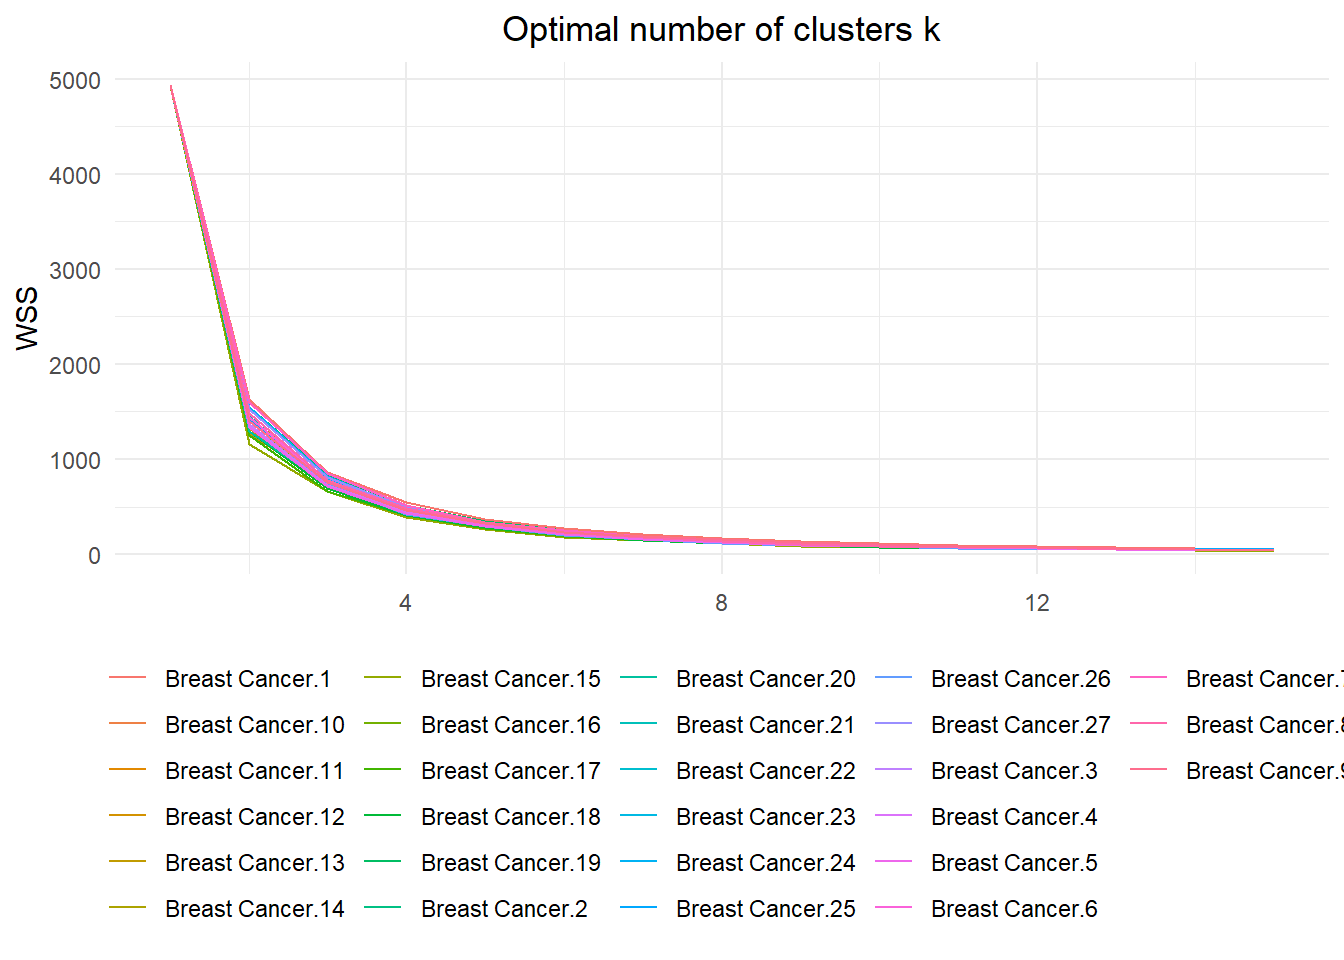
\includegraphics{finalReport_für_PDF_files/figure-latex/unnamed-chunk-10-1}

\}

\textbackslash caption\{\emph{Fig. 3} Expression values of 12 selected
driver mutations\}\label{fig:unnamed-chunk-10}
\textbackslash end\{figure\}

Some of these genes were not followed up further due to being known as
tumor suppressor genes (e.g.~RB1, TP53). This was because our approach
opts for targets reducing cell viability after a knockdown. A knockdown
of a tumor suppressor gene, even if it is mutated, will rarely have a
negative effect on cell viability. This makes genes associated with
tumor suppressor genes useless for an inhibitory drug and therefore not
appropriate for our analysis.

\hypertarget{generation-of-the-mutimpact-matrix}{%
\subsubsection{Generation of the mutImpact
matrix}\label{generation-of-the-mutimpact-matrix}}

Every mutation has an impact on cell viability. In our analysis we have
to distinguish not only between single mutations, we also have to
evaluate different mutations in our cell lines ``working together'' and
making every cell line different in its characteristics. In order to
gain an overview of these characteristics, we will generate a matrix,
showing the effect on viability, caused by a single mutation, in every
cell line. The generated matrix will be called \texttt{mutImpact}
matrix.

Therefore, the BCCL\_kd.ceres matrix containing CERES scores for all
genes in breast cancer cell lines was used as a template and the cell
line IDs were added as column names creating a pre\_mutImpact matrix. An
empty matrix was generated comprising 17634 rows and 28 columns matching
the number of genes per cell line and the number of breast cancer cell
lines, respectively.

Subsequently, CERES scores of genes, which were not mutated in a given
cell line, were replaced with \texttt{NA} by implementing an ``if
statement''. This statement included the enquiry whether the gene ID is
present in the list of mutated genes of a considered cell line and in
case the condition was met the CERES score was maintained. If
\texttt{FALSE} was returned, the CERES score of the gene was replaced
with \texttt{NA} for the considered cell line.

\begin{Shaded}
\begin{Highlighting}[]
\CommentTok{#Generate pre_mutImpact matrix containing all CERES values and with IDs as column names }
\NormalTok{pre_mutImpact <-}\StringTok{ }\NormalTok{BCCL_kd.ceres}
\KeywordTok{colnames}\NormalTok{(pre_mutImpact)<-tPatients_ID}

\CommentTok{#Generate empty mutImpact matrix}
\NormalTok{mutImpact <-}\StringTok{ }\KeywordTok{matrix}\NormalTok{(, }\DataTypeTok{nrow =} \DecValTok{17634}\NormalTok{, }\DataTypeTok{ncol =} \DecValTok{28}\NormalTok{)}
\KeywordTok{colnames}\NormalTok{(mutImpact)<-}\KeywordTok{colnames}\NormalTok{(pre_mutImpact)}
\KeywordTok{rownames}\NormalTok{(mutImpact)<-}\KeywordTok{rownames}\NormalTok{(pre_mutImpact)}

\CommentTok{#Fill mutImpact matrix with values}
\ControlFlowTok{for}\NormalTok{ (j }\ControlFlowTok{in} \DecValTok{1}\OperatorTok{:}\KeywordTok{ncol}\NormalTok{(pre_mutImpact))\{}
\NormalTok{  lineID <-}\StringTok{ }\KeywordTok{colnames}\NormalTok{(pre_mutImpact)[j] }\CommentTok{#Select a column-name = cell line}
  \ControlFlowTok{for}\NormalTok{ (i }\ControlFlowTok{in} \DecValTok{1}\OperatorTok{:}\KeywordTok{nrow}\NormalTok{(pre_mutImpact))\{}
\NormalTok{    GOI <-}\StringTok{ }\KeywordTok{rownames}\NormalTok{(pre_mutImpact)[i] }\CommentTok{#Select a gene}
    \ControlFlowTok{if}\NormalTok{ (GOI }\OperatorTok\StringTok{ }\NormalTok{BCCL_Mutation[[lineID]]}\OperatorTok{$}\NormalTok{Hugo_Symbol)\{}
\NormalTok{      mutImpact[i, j] <-}\StringTok{ }\NormalTok{pre_mutImpact[i, j]}
\NormalTok{    \} }\ControlFlowTok{else}\NormalTok{ \{}
\NormalTok{      mutImpact[i, j] <-}\StringTok{ }\OtherTok{NA}
\NormalTok{    \}}\CommentTok{#Replace CERES value with NA in case the gene is not mutated}
\NormalTok{  \}}
\NormalTok{\}}

\CommentTok{#Have a look at the mutImpact matrix}
\KeywordTok{View}\NormalTok{(}\KeywordTok{head}\NormalTok{(}\KeywordTok{as.data.frame}\NormalTok{(mutImpact)))}
\end{Highlighting}
\end{Shaded}

\hypertarget{selection-of-driver-mutations}{%
\subsection{Selection of driver
mutations}\label{selection-of-driver-mutations}}

\hypertarget{identification-of-driver-mutations-using-k-means-clustering-of-ceres-scores}{%
\subsubsection{Identification of driver mutations using k means
clustering of CERES
scores}\label{identification-of-driver-mutations-using-k-means-clustering-of-ceres-scores}}

In order to verify our selection of driver mutations from literature
research, k means clustering of CERES scores was performed. Suitable
driver mutations were expected to be found in the same cluster based on
scaled CERES scores, since in this way equal effects on cell viability
can be ensured.

K means clustering was performed with all genes mutated at least once in
28 cell line samples and whose CERES score is not greater than zero. For
this, all genes with only NA values (hence, not mutated in the
\texttt{MutImpact\ Matrix}) were removed. A new dataframe
\texttt{BCCL\_kd.ceres\_2}was generated containing all 28 CERES scores
for each gene, with gene names in the first column. These names were
compared to the rownames of \texttt{mutImpact\_c} to generate the
\texttt{BCCL\_kd.ceres\_3} dataframe. The resulting dataframe contains
CERES scores of all genes mutated at least once for each breast cell
cancer lines. Subsequently, the average mean CERES score for each gene
was computed using the \texttt{rowMeans} function and stored in the last
column. To carry out this step, the column \texttt{rownameskdc2} was
removed. Finally, all genes with CERES scores \textgreater{} 0 were
deleted. The final \texttt{BCCL\_kd.ceres\_3} dataframe consisted of
4934 genes mutated at least once in the 28 breast cancer cell lines and
with mean CERES scores equal to or below 0.

\begin{Shaded}
\begin{Highlighting}[]
\CommentTok{#Selecting only genes mutated at least once and with Ceres <= 0}
\NormalTok{mutImpact_c =}\StringTok{ }\NormalTok{mutImpact[}\KeywordTok{rowSums}\NormalTok{(}\KeywordTok{is.na}\NormalTok{(mutImpact)) }\OperatorTok{!=}\StringTok{ }\KeywordTok{ncol}\NormalTok{(mutImpact),] }\CommentTok{#Remove all genes with all NA values}
\NormalTok{rownamesmutImpc =}\StringTok{ }\KeywordTok{rownames}\NormalTok{(mutImpact_c)}
\NormalTok{mutImpact_c =}\StringTok{ }\KeywordTok{cbind}\NormalTok{(rownamesmutImpc, mutImpact_c[,}\DecValTok{2}\OperatorTok{:}\KeywordTok{ncol}\NormalTok{(mutImpact_c)]) }\CommentTok{#Insert new column with row names}
\KeywordTok{dim}\NormalTok{(mutImpact_c) }\CommentTok{#Check gene reduction }
\end{Highlighting}
\end{Shaded}

\begin{verbatim}
## [1] 7810   28
\end{verbatim}

\begin{Shaded}
\begin{Highlighting}[]
\NormalTok{rownameskdc2 =}\StringTok{ }\KeywordTok{rownames}\NormalTok{(BCCL_kd.ceres) }\CommentTok{#Define vector of BCCL_kd.ceres rownames }

\NormalTok{BCCL_kd.ceres_}\DecValTok{2}\NormalTok{ =}\StringTok{ }\KeywordTok{cbind}\NormalTok{(rownameskdc2, BCCL_kd.ceres[,}\DecValTok{2}\OperatorTok{:}\KeywordTok{ncol}\NormalTok{(BCCL_kd.ceres)]) }\CommentTok{#Insert new column with row names}
\NormalTok{BCCL_kd.ceres_}\DecValTok{3}\NormalTok{ =}\StringTok{ }\NormalTok{BCCL_kd.ceres_}\DecValTok{2}\NormalTok{[BCCL_kd.ceres_}\DecValTok{2}\NormalTok{[,}\StringTok{"rownameskdc2"}\NormalTok{] }\OperatorTok\StringTok{  }\NormalTok{mutImpact_c[,}\StringTok{"rownamesmutImpc"}\NormalTok{],][,}\OperatorTok{-}\KeywordTok{c}\NormalTok{(}\DecValTok{1}\NormalTok{)]}
\NormalTok{BCCL_kd.ceres_}\DecValTok{3}\NormalTok{ =}\StringTok{ }\KeywordTok{cbind}\NormalTok{(BCCL_kd.ceres_}\DecValTok{3}\NormalTok{, }\KeywordTok{rowMeans}\NormalTok{(BCCL_kd.ceres_}\DecValTok{3}\NormalTok{))[}\KeywordTok{rowMeans}\NormalTok{(}\KeywordTok{cbind}\NormalTok{(BCCL_kd.ceres_}\DecValTok{3}\NormalTok{, }\KeywordTok{rowMeans}\NormalTok{(BCCL_kd.ceres_}\DecValTok{3}\NormalTok{)))}\OperatorTok{<=}\StringTok{ }\DecValTok{0}\NormalTok{,] }\CommentTok{#Deletion of genes with CERES > 0}
\KeywordTok{dim}\NormalTok{(BCCL_kd.ceres_}\DecValTok{3}\NormalTok{)}
\end{Highlighting}
\end{Shaded}

\begin{verbatim}
## [1] 4934   28
\end{verbatim}

In preparation of k means clustering, the column containing average
CERES scores for each gene was removed (new dataframe
\texttt{BCCL\_kd.ceresKS}) and the optimal number of k clusters
identified. For each column (cell sample) of the dataframe, the values
were scaled. For cluster numbers between 2 and 15 the within sum of
squares (WSS) for each cell sample was calculated and stored as a
separate dataframe. To ensure that the same result is obtained each time
the code is run, the set.seed(1234) function was used.

\begin{Shaded}
\begin{Highlighting}[]
\CommentTok{#Determine optimal cluster number k}
\NormalTok{BCCL_kd.ceresKS =}\StringTok{ }\NormalTok{BCCL_kd.ceres_}\DecValTok{3}\NormalTok{[,}\OperatorTok{-}\KeywordTok{c}\NormalTok{(}\DecValTok{28}\NormalTok{)] }\CommentTok{#Remove column of average CERES value column }

\NormalTok{CERES_Optimal_K <-}\StringTok{ }\ControlFlowTok{function}\NormalTok{(BCCL_kd.ceresKS, specifier) \{}
\NormalTok{  output <-}\StringTok{ }\KeywordTok{lapply}\NormalTok{(}\DecValTok{1}\OperatorTok{:}\KeywordTok{ncol}\NormalTok{(BCCL_kd.ceresKS), }\ControlFlowTok{function}\NormalTok{(a)\{}
\NormalTok{   df <-}\StringTok{ }\KeywordTok{scale}\NormalTok{(BCCL_kd.ceresKS[,a]) }\CommentTok{#Pick one column of input data and scale }
\NormalTok{   wss <-(}\KeywordTok{nrow}\NormalTok{(df}\DecValTok{-1}\NormalTok{))}\OperatorTok{*}\KeywordTok{sum}\NormalTok{(}\KeywordTok{apply}\NormalTok{(df,}\DecValTok{2}\NormalTok{,var)) }\CommentTok{#Define method of wss computation }
   \ControlFlowTok{for}\NormalTok{ (i }\ControlFlowTok{in} \DecValTok{2}\OperatorTok{:}\DecValTok{15}\NormalTok{)\{ }\CommentTok{#For k between 2 and 15}
     \KeywordTok{set.seed}\NormalTok{(}\DecValTok{1234}\NormalTok{) }\CommentTok{#To ensure reproducability of results }
\NormalTok{     wss[i] <-}\StringTok{ }\KeywordTok{sum}\NormalTok{(}\KeywordTok{kmeans}\NormalTok{(df, }\DataTypeTok{centers =}\NormalTok{ i)}\OperatorTok{$}\NormalTok{withinss)}
\NormalTok{     \} }
   \KeywordTok{return}\NormalTok{(wss)}
\NormalTok{  \})}
\KeywordTok{names}\NormalTok{ (output) <-}\StringTok{ }\KeywordTok{colnames}\NormalTok{(BCCL_kd.ceresKS) }\CommentTok{#Rename the output }
\KeywordTok{return}\NormalTok{(output)}
\NormalTok{\}}

\NormalTok{BCCL_kd.ceres_optKS <-}\StringTok{ }\KeywordTok{CERES_Optimal_K}\NormalTok{(BCCL_kd.ceresKS, }\StringTok{"CERES Optimal Clusters k"}\NormalTok{) }
\end{Highlighting}
\end{Shaded}

To enable the plotting of within sum square values for clusters from 2
to 15 for each breast cancer cell, each vector was individually picked
and formatted into a dataframe. The cell sample name was then added as a
label in a new column ``Cell\_Sample'' and the cluster numbers from 2 to
15 in the column ``OptimalK''. The output of this lapply function
(\texttt{optimalKprocessedData}), a list of 28 dataframes, was then
combined into one and columns renamed accordingly. Subsequently, the
ggplot function was used to plot all data stored in
\texttt{optimalKprocessedData} in one plot.

\begin{Shaded}
\begin{Highlighting}[]
\CommentTok{#Plotting wss function }
\NormalTok{optimalKprocessedData <-}\StringTok{ }\KeywordTok{lapply}\NormalTok{(}\KeywordTok{seq_along}\NormalTok{(BCCL_kd.ceres_optKS), }\ControlFlowTok{function}\NormalTok{(a)\{}
\NormalTok{  dtPicker <-}\StringTok{ }\KeywordTok{as.data.frame}\NormalTok{(BCCL_kd.ceres_optKS[[a]]) }\CommentTok{#One vector picked and formatted into dataframe}
\NormalTok{  dtPicker}\OperatorTok{$}\NormalTok{Cell_Sample <-}\StringTok{ }\KeywordTok{names}\NormalTok{(BCCL_kd.ceres_optKS)[a] }\CommentTok{#Sample added as label}
\NormalTok{  dtPicker}\OperatorTok{$}\NormalTok{OptimalK <-}\StringTok{ }\DecValTok{1}\OperatorTok{:}\KeywordTok{nrow}\NormalTok{(dtPicker) }
  \KeywordTok{return}\NormalTok{(dtPicker)}
\NormalTok{\})}

\NormalTok{optimalKprocessedData <-}\StringTok{ }\KeywordTok{as.data.frame}\NormalTok{(}\KeywordTok{do.call}\NormalTok{(}\StringTok{"rbind"}\NormalTok{,optimalKprocessedData)) }\CommentTok{#Output into dataframe}
\KeywordTok{colnames}\NormalTok{(optimalKprocessedData) <-}\StringTok{ }\KeywordTok{c}\NormalTok{(}\StringTok{"WSS"}\NormalTok{, }\StringTok{"Cell_Sample"}\NormalTok{, }\StringTok{"OptimalK"}\NormalTok{) }\CommentTok{#Renaming columns}

\CommentTok{#Using ggplot to plot output }
\KeywordTok{ggplot}\NormalTok{(}\DataTypeTok{data =}\NormalTok{ optimalKprocessedData, }\KeywordTok{aes}\NormalTok{(}\DataTypeTok{x=}\NormalTok{OptimalK, }\DataTypeTok{y=}\NormalTok{WSS)) }\OperatorTok{+}
\StringTok{  }\KeywordTok{geom_line}\NormalTok{(}\KeywordTok{aes}\NormalTok{(}\DataTypeTok{color=}\NormalTok{Cell_Sample)) }\OperatorTok{+}
\StringTok{  }\KeywordTok{labs}\NormalTok{(}\DataTypeTok{title =} \StringTok{'Optimal number of clusters k'}\NormalTok{, }\DataTypeTok{x =} \StringTok{'Number of clusters'}\NormalTok{, }\DataTypeTok{y =} \StringTok{'WSS'}\NormalTok{) }\OperatorTok{+}
\StringTok{  }\KeywordTok{theme_minimal}\NormalTok{() }\OperatorTok{+}
\StringTok{           }\KeywordTok{theme}\NormalTok{(}\DataTypeTok{legend.position =}\StringTok{'none'}\NormalTok{,}
                  \DataTypeTok{plot.title =} \KeywordTok{element_text}\NormalTok{(}\DataTypeTok{hjust =} \FloatTok{0.5}\NormalTok{),}
                  \DataTypeTok{axis.text.x =} \KeywordTok{element_text}\NormalTok{(}\DataTypeTok{angle =} \DecValTok{0}\NormalTok{, }\DataTypeTok{vjust =} \DecValTok{0}\NormalTok{, }\DataTypeTok{hjust=}\FloatTok{0.5}\NormalTok{),}
                  \DataTypeTok{legend.title=} \KeywordTok{element_blank}\NormalTok{(),}
                  \DataTypeTok{axis.title.x =} \KeywordTok{element_blank}\NormalTok{(),}
                  \DataTypeTok{strip.text.y =} \KeywordTok{element_text}\NormalTok{(}\DataTypeTok{angle =} \DecValTok{0}\NormalTok{))}
\end{Highlighting}
\end{Shaded}

\textbackslash begin\{figure\}

\{\centering \includegraphics{finalReport_für_PDF_files/figure-latex/unnamed-chunk-14-1}

\}

\textbackslash caption\{\emph{Fig. 4} Optimal number of clusters k using
WSS of each BBCLs\}\label{fig:unnamed-chunk-14}
\textbackslash end\{figure\}

From this plot it is evident that the optimal cluster number lies
between 2 and 4 if the elbow method is applied. To verify this result
and to determine a precise number of optimal cluster, an alternative
plotting method calculating the average WSS for cluster numbers between
2 and 15 for all 28 cell samples was performed and with this the optimal
cluster number k was identified to be 4. Thus, k means clustering of the
data stored in \texttt{BCCL\_kd.ceres\_3} was performed with 10
iterations. The following cluster plot was generated.

\begin{Shaded}
\begin{Highlighting}[]
\NormalTok{km_CERES=}\StringTok{ }\KeywordTok{kmeans}\NormalTok{(}\DataTypeTok{x =}\NormalTok{ BCCL_kd.ceres_}\DecValTok{3}\NormalTok{, }\DataTypeTok{centers =} \DecValTok{4}\NormalTok{, }\DataTypeTok{nstart =} \DecValTok{10}\NormalTok{)}
\KeywordTok{table}\NormalTok{(km_CERES}\OperatorTok{$}\NormalTok{cluster)}
\end{Highlighting}
\end{Shaded}

\begin{verbatim}
## 
##    1    2    3    4 
##  490 3028 1171  245
\end{verbatim}

\begin{Shaded}
\begin{Highlighting}[]
\KeywordTok{fviz_cluster}\NormalTok{(km_CERES, }\DataTypeTok{data=}\NormalTok{BCCL_kd.ceres_}\DecValTok{3}\NormalTok{, }\DataTypeTok{labelsize =} \DecValTok{6}\NormalTok{) }\CommentTok{#Plotting clusters}
\end{Highlighting}
\end{Shaded}

\textbackslash begin\{figure\}

\{\centering \includegraphics{finalReport_für_PDF_files/figure-latex/unnamed-chunk-15-1}

\}

\textbackslash caption\{\emph{Fig. 5} K means cluster
plot\}\label{fig:unnamed-chunk-15} \textbackslash end\{figure\}

In order to verify our selection of driver mutations from literature,
the cluster number of each driver mutation was identified. All selected
driver mutations from literature,``ERBB2'', ``MYCBP'', ``PARP10'' and
``PIK3CA'' were colocalized in cluster 3, hence with similar CERES
scores, with the exception of ``CCND'' and ``ERBBIP''. While ``CCND''
was removed in the filtering process (removal of not mutated genes and
genes with CERES \textgreater0) and no longer found
in\texttt{BCCL\_kd.ceres\_3}, ``ERBB2IP'' was found in cluster 4. For
these reasons the two mentioned mutations were excluded from further
analysis, to leave only ``ERBB2'', ``MYCBP'', ``PARP10'' and ``PIK3CA''
as selected driver mutations.

\begin{Shaded}
\begin{Highlighting}[]
\NormalTok{driver_mut <-}\StringTok{ }\KeywordTok{c}\NormalTok{(}\StringTok{"ERBB2"}\NormalTok{,}\StringTok{"ERBB2IP"}\NormalTok{, }\StringTok{"MYCBP"}\NormalTok{, }\StringTok{"PARP10"}\NormalTok{, }\StringTok{"PIK3CA"}\NormalTok{) }\CommentTok{#Enter driver mutations}
\NormalTok{CheckKmNumber <-}\StringTok{ }\KeywordTok{as.data.frame}\NormalTok{(}\KeywordTok{sapply}\NormalTok{(}\KeywordTok{seq_along}\NormalTok{(driver_mut), }\ControlFlowTok{function}\NormalTok{(a)\{}
\NormalTok{  out <-}\StringTok{ }\NormalTok{km_CERES}\OperatorTok{$}\NormalTok{cluster[driver_mut[a]]}
  \KeywordTok{return}\NormalTok{(out)}
\NormalTok{\}))}

\KeywordTok{colnames}\NormalTok{(CheckKmNumber) <-}\StringTok{ "Cluster number"}
\KeywordTok{View}\NormalTok{(CheckKmNumber)}
\end{Highlighting}
\end{Shaded}

Since our approach defined SSTs as genes expected to interact
synergistically with the corresponding driver mutation in promoting cell
viability, similar CERES scores were expected. Thus all potential SSTs
candidates were expected to be found in cluster 3 as well. This
characteristic of SSTs will be checked in section 3.3.2. A dataframe
\texttt{data\_clus\_3}was subsequently generated to contain all 1148
genes colocalized with driver mutations in cluster 3.

\begin{Shaded}
\begin{Highlighting}[]
\NormalTok{data_cluster =}\StringTok{ }\KeywordTok{as.data.frame}\NormalTok{(km_CERES}\OperatorTok{$}\NormalTok{cluster)}
\KeywordTok{rownames}\NormalTok{(data_cluster) =}\StringTok{ }\KeywordTok{rownames}\NormalTok{(BCCL_kd.ceres_}\DecValTok{3}\NormalTok{)}
\NormalTok{data_clus_}\DecValTok{3}\NormalTok{ =}\StringTok{ }\NormalTok{BCCL_kd.ceres_}\DecValTok{3}\NormalTok{[data_cluster }\OperatorTok{==}\StringTok{ }\DecValTok{3}\NormalTok{,] }\CommentTok{#Dataframe with all 1148 genes in same cluster as driver mutations }
\end{Highlighting}
\end{Shaded}

A further dataframe \texttt{data\_clus\_3e} was subsequently generated
labelling the four driver mutations in a separate column, by
implementing an ``if'' loop. If a rowname of \texttt{data\_clus\_3e}was
found in a previously created vector containing driver mutations names
(\texttt{drivermut}), it was labelled as ``driver mutation''. Otherwise
genes were labelled as ``no driver mutation''.

\begin{Shaded}
\begin{Highlighting}[]
\NormalTok{drivermut =}\StringTok{  }\KeywordTok{c}\NormalTok{(}\StringTok{"ERBB2"}\NormalTok{,}\StringTok{"MYCBP"}\NormalTok{, }\StringTok{"PARP10"}\NormalTok{, }\StringTok{"PIK3CA"}\NormalTok{) }\CommentTok{#Create vector with driver mutation names}

\NormalTok{data_clus_3e =}\StringTok{ }\NormalTok{data_clus_}\DecValTok{3}
\NormalTok{data_clus_3e[}\StringTok{"Driver mutation"}\NormalTok{] <-}\StringTok{ }\KeywordTok{sapply}\NormalTok{(}\DecValTok{1}\OperatorTok{:}\KeywordTok{nrow}\NormalTok{(data_clus_}\DecValTok{3}\NormalTok{), }\ControlFlowTok{function}\NormalTok{(j)\{}
     \ControlFlowTok{if}\NormalTok{(}\KeywordTok{rownames}\NormalTok{(data_clus_3e)[j] }\OperatorTok\StringTok{ }\NormalTok{drivermut)\{ }
\NormalTok{         data_clus_3e[j,}\DecValTok{1}\NormalTok{] =}\StringTok{ "driver mutation"}
\NormalTok{     \} }\ControlFlowTok{else}\NormalTok{ \{}
\NormalTok{         data_clus_3e[j,}\DecValTok{1}\NormalTok{] =}\StringTok{ "no driver mutation"}
\NormalTok{     \}}
\NormalTok{  \}) }\CommentTok{#Labelling driver mutations with their DV status in data_clus_3e }
\end{Highlighting}
\end{Shaded}

\hypertarget{data-visualisation-of-ceres-and-tpm-values-for-selected-driver-mutations}{%
\subsubsection{Data visualisation of CERES and TPM values for selected
driver
mutations}\label{data-visualisation-of-ceres-and-tpm-values-for-selected-driver-mutations}}

CERES scores and expression in TPM values for the selected four driver
mutations were visualised as box and whisker plots. Following the
generation of the \texttt{GOI\_X} dataframe containing either CERES or
TPM values for the four mutations, the data was reshaped to contain two
columns. One column being ``variable'' with the names of driver
mutations, the other ``value'' with the corresponding CERES or TPM
value. The ggplot function, part of the ggplot2 package, was used to
plot the following box an whisker plots.

\begin{Shaded}
\begin{Highlighting}[]
\CommentTok{#CERES_boxplot}
\NormalTok{GOI=}\StringTok{ }\NormalTok{BCCL_kd.ceres[}\KeywordTok{c}\NormalTok{(}\StringTok{"ERBB2"}\NormalTok{,}\StringTok{"MYCBP"}\NormalTok{, }\StringTok{"PARP10"}\NormalTok{, }\StringTok{"PIK3CA"}\NormalTok{),]}
\NormalTok{CERES_driver_mut=}\StringTok{ }\KeywordTok{melt}\NormalTok{(GOI)}
\end{Highlighting}
\end{Shaded}

\begin{verbatim}
## No id variables; using all as measure variables
\end{verbatim}

\begin{Shaded}
\begin{Highlighting}[]
\NormalTok{CERES_driver_mut}\OperatorTok{$}\NormalTok{variable=}\KeywordTok{rep}\NormalTok{(}\KeywordTok{c}\NormalTok{(}\StringTok{"ERBB2"}\NormalTok{,}\StringTok{"MYCBP"}\NormalTok{, }\StringTok{"PARP10"}\NormalTok{, }\StringTok{"PIK3CA"}\NormalTok{), }\KeywordTok{ncol}\NormalTok{(GOI)) }\CommentTok{#replication of driver mutation names as often as number of GOI columns}

\NormalTok{CERES_boxplot =}\StringTok{ }\KeywordTok{ggplot}\NormalTok{(CERES_driver_mut, }\KeywordTok{aes}\NormalTok{(}\DataTypeTok{x =}\NormalTok{ variable, }\DataTypeTok{y =}\NormalTok{ value)) }\OperatorTok{+}
\StringTok{       }\KeywordTok{geom_boxplot}\NormalTok{(}\KeywordTok{aes}\NormalTok{(}\DataTypeTok{fill=}\NormalTok{variable), }\DataTypeTok{outlier.alpha =} \FloatTok{0.7}\NormalTok{,}
                     \DataTypeTok{outlier.colour =} \StringTok{"grey"}\NormalTok{, }\DataTypeTok{outlier.shape =} \DecValTok{20}\NormalTok{, }\DataTypeTok{outlier.size =} \DecValTok{2}\NormalTok{) }\OperatorTok{+}
\StringTok{        }\KeywordTok{labs}\NormalTok{(}\DataTypeTok{title =} \StringTok{'CERES scores of selected driver mutations'}\NormalTok{, }\DataTypeTok{x =} \StringTok{'Selected driver mutations'}\NormalTok{, }\DataTypeTok{y =} \StringTok{'CERES scores'}\NormalTok{) }\OperatorTok{+}
\StringTok{            }\KeywordTok{theme_minimal}\NormalTok{() }\OperatorTok{+}
\StringTok{            }\KeywordTok{geom_jitter}\NormalTok{(}\DataTypeTok{width =} \FloatTok{0.2}\NormalTok{) }\OperatorTok{+}
\StringTok{            }\KeywordTok{scale_fill_manual}\NormalTok{(}\DataTypeTok{values =} \KeywordTok{wes_palette}\NormalTok{(}\StringTok{"Royal2"}\NormalTok{, }\DataTypeTok{n=}\DecValTok{4}\NormalTok{)) }\OperatorTok{+}
\StringTok{            }\KeywordTok{theme}\NormalTok{(}\DataTypeTok{legend.position =}\StringTok{'none'}\NormalTok{,}
                  \DataTypeTok{plot.title =} \KeywordTok{element_text}\NormalTok{(}\DataTypeTok{hjust =} \FloatTok{0.4}\NormalTok{),}
                  \DataTypeTok{axis.text.x =} \KeywordTok{element_text}\NormalTok{(}\DataTypeTok{angle =} \DecValTok{0}\NormalTok{, }\DataTypeTok{vjust =} \DecValTok{0}\NormalTok{, }\DataTypeTok{hjust=}\FloatTok{0.5}\NormalTok{),}
                  \DataTypeTok{legend.title=} \KeywordTok{element_blank}\NormalTok{(),}
                  \DataTypeTok{axis.title.x =} \KeywordTok{element_text}\NormalTok{(),}
                  \DataTypeTok{strip.text.y =} \KeywordTok{element_text}\NormalTok{(}\DataTypeTok{angle =} \DecValTok{0}\NormalTok{))}
\NormalTok{CERES_boxplot}
\end{Highlighting}
\end{Shaded}

\textbackslash begin\{figure\}

\{\centering 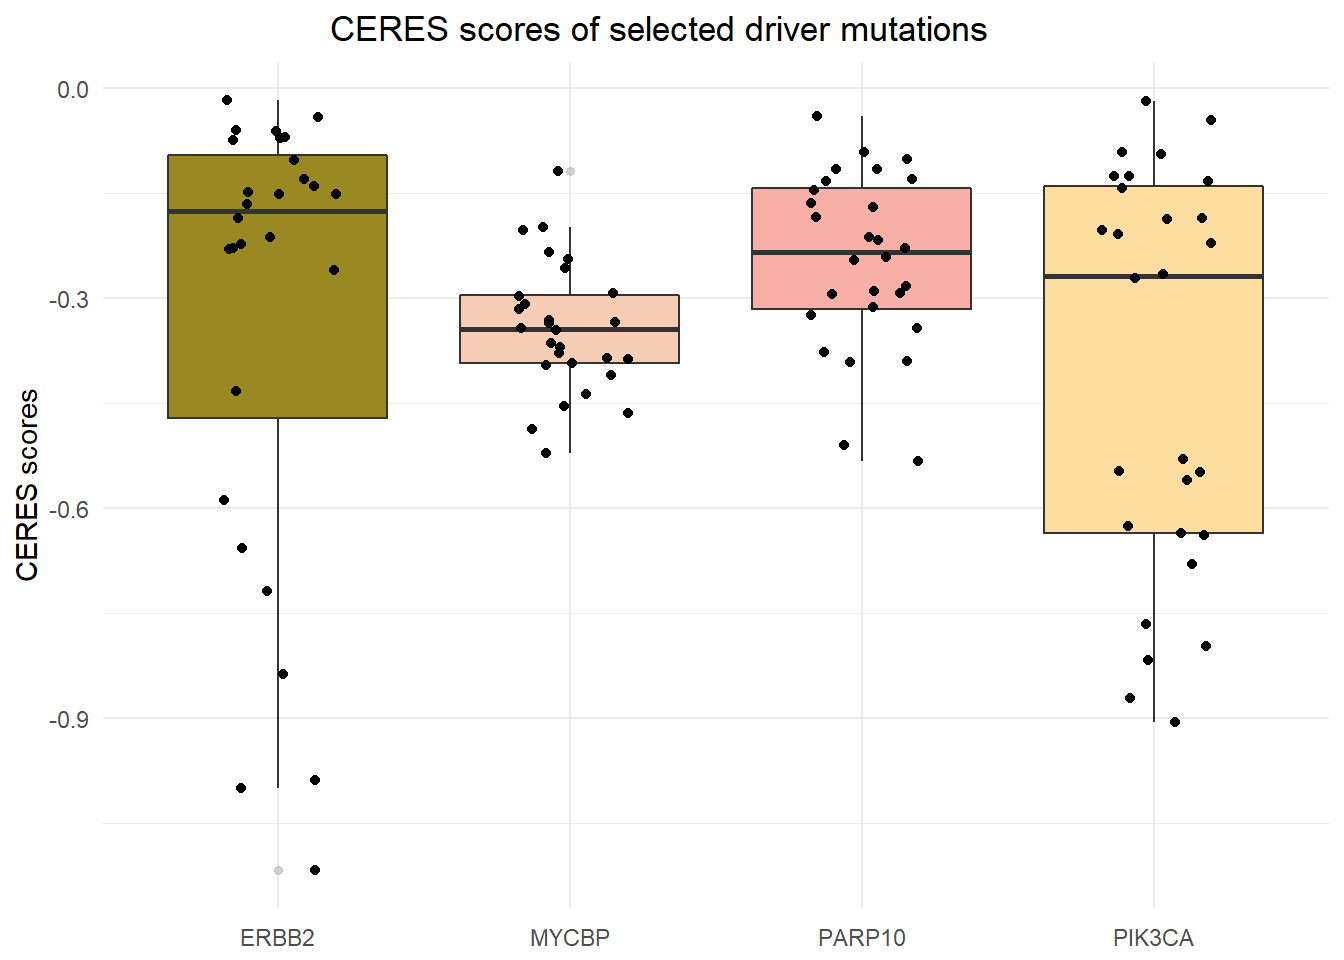
\includegraphics{finalReport_für_PDF_files/figure-latex/data visualisation-1}

\}

\textbackslash caption\{\emph{Fig. 6} Boxplot of CERES and Expression
values of selected driver mutations\}\label{fig:data visualisation1}
\textbackslash end\{figure\}

\begin{Shaded}
\begin{Highlighting}[]
\CommentTok{#Expression_boxplot}
\NormalTok{GOI_Exp=}\StringTok{ }\NormalTok{BCCL_Expression[}\KeywordTok{c}\NormalTok{(}\StringTok{"ERBB2"}\NormalTok{,}\StringTok{"MYCBP"}\NormalTok{, }\StringTok{"PARP10"}\NormalTok{, }\StringTok{"PIK3CA"}\NormalTok{),]}
\NormalTok{Expression_driver_mut=}\StringTok{ }\KeywordTok{melt}\NormalTok{(GOI_Exp)}
\end{Highlighting}
\end{Shaded}

\begin{verbatim}
## No id variables; using all as measure variables
\end{verbatim}

\begin{Shaded}
\begin{Highlighting}[]
\NormalTok{Expression_driver_mut}\OperatorTok{$}\NormalTok{variable=}\KeywordTok{rep}\NormalTok{(}\KeywordTok{c}\NormalTok{(}\StringTok{"ERBB2"}\NormalTok{,}\StringTok{"MYCBP"}\NormalTok{, }\StringTok{"PARP10"}\NormalTok{, }\StringTok{"PIK3CA"}\NormalTok{), }\KeywordTok{ncol}\NormalTok{(GOI_Exp))}

\NormalTok{Expression_boxplot =}\StringTok{ }\KeywordTok{ggplot}\NormalTok{(Expression_driver_mut, }\KeywordTok{aes}\NormalTok{(}\DataTypeTok{x =}\NormalTok{ variable, }\DataTypeTok{y =}\NormalTok{ value)) }\OperatorTok{+}
\StringTok{       }\KeywordTok{geom_boxplot}\NormalTok{(}\KeywordTok{aes}\NormalTok{(}\DataTypeTok{fill=}\NormalTok{variable), }\DataTypeTok{outlier.alpha =} \FloatTok{0.7}\NormalTok{,}
                     \DataTypeTok{outlier.colour =} \StringTok{"grey"}\NormalTok{, }\DataTypeTok{outlier.shape =} \DecValTok{20}\NormalTok{, }\DataTypeTok{outlier.size =} \DecValTok{2}\NormalTok{) }\OperatorTok{+}
\StringTok{        }\KeywordTok{labs}\NormalTok{(}\DataTypeTok{title =} \StringTok{'Transcripts per million (TPM) of selected driver mutations'}\NormalTok{, }\DataTypeTok{x =} \StringTok{'Selected driver mutations'}\NormalTok{, }\DataTypeTok{y =} \StringTok{'Transcripts per million [TPM]'}\NormalTok{) }\OperatorTok{+}
\StringTok{            }\KeywordTok{theme_minimal}\NormalTok{() }\OperatorTok{+}
\StringTok{            }\KeywordTok{geom_jitter}\NormalTok{(}\DataTypeTok{width =} \FloatTok{0.2}\NormalTok{) }\OperatorTok{+}
\StringTok{            }\KeywordTok{scale_fill_manual}\NormalTok{(}\DataTypeTok{values=}\KeywordTok{wes_palette}\NormalTok{(}\StringTok{"Royal2"}\NormalTok{, }\DataTypeTok{n=}\DecValTok{4}\NormalTok{)) }\OperatorTok{+}
\StringTok{            }\KeywordTok{theme}\NormalTok{(}\DataTypeTok{legend.position =}\StringTok{'none'}\NormalTok{,}
                  \DataTypeTok{plot.title =} \KeywordTok{element_text}\NormalTok{(}\DataTypeTok{hjust =} \FloatTok{0.4}\NormalTok{),}
                  \DataTypeTok{axis.text.x =} \KeywordTok{element_text}\NormalTok{(}\DataTypeTok{angle =} \DecValTok{0}\NormalTok{, }\DataTypeTok{vjust =} \DecValTok{0}\NormalTok{, }\DataTypeTok{hjust=}\FloatTok{0.5}\NormalTok{),}
                  \DataTypeTok{legend.title=} \KeywordTok{element_blank}\NormalTok{(),}
                  \DataTypeTok{axis.title.x =} \KeywordTok{element_text}\NormalTok{(),}
                  \DataTypeTok{strip.text.y =} \KeywordTok{element_text}\NormalTok{(}\DataTypeTok{angle =} \DecValTok{0}\NormalTok{))}
\NormalTok{Expression_boxplot}
\end{Highlighting}
\end{Shaded}

\textbackslash begin\{figure\}

\{\centering 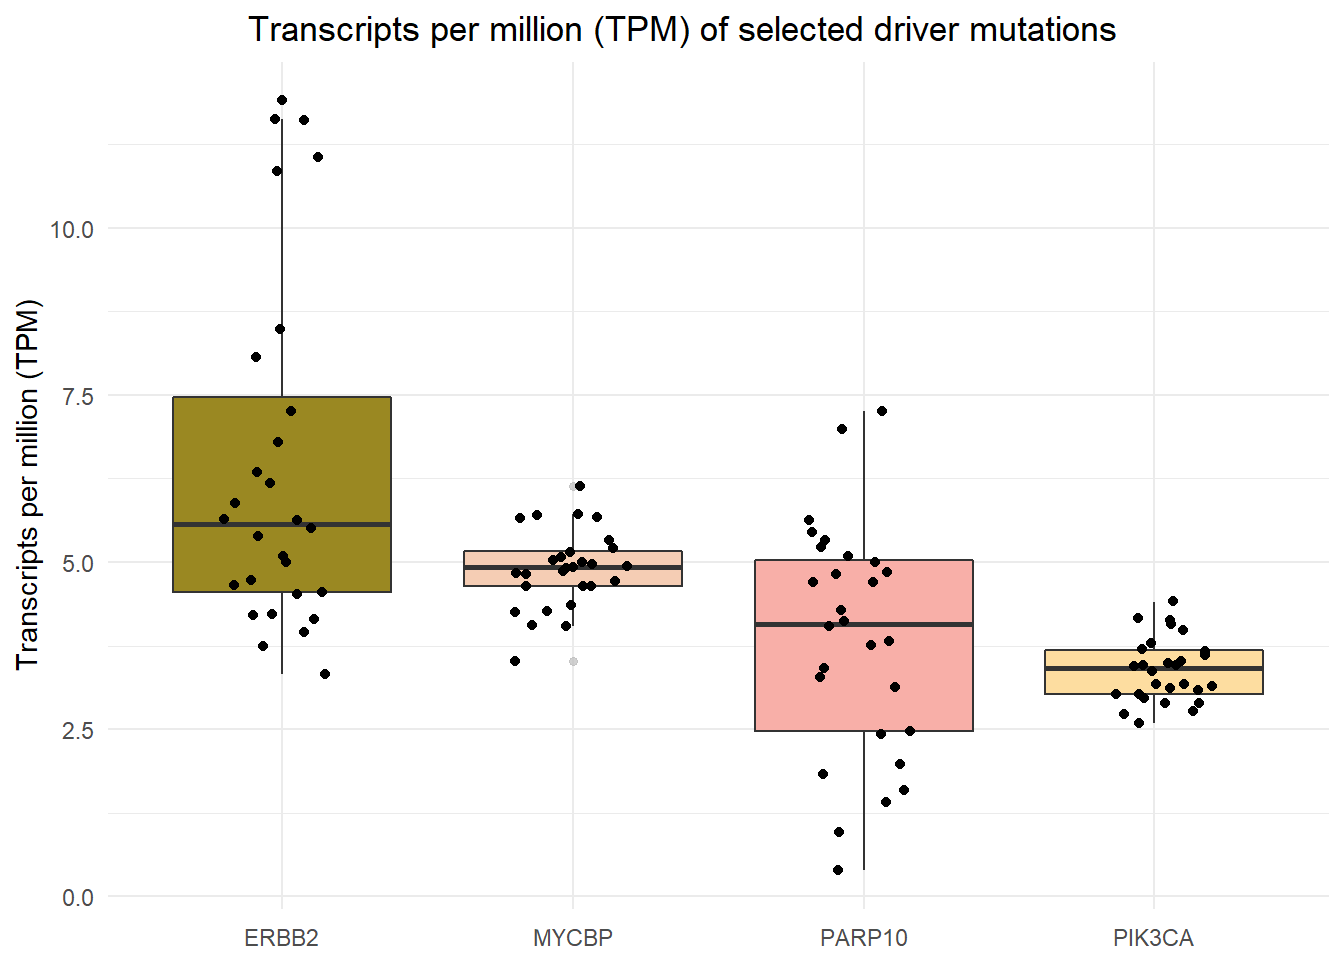
\includegraphics{finalReport_für_PDF_files/figure-latex/data visualisation-2}

\}

\textbackslash caption\{\emph{Fig. 6} Boxplot of CERES and Expression
values of selected driver mutations\}\label{fig:data visualisation2}
\textbackslash end\{figure\}

The box- and whisker plot of CERES scores reveal MYCBP as the most
essential driver gene for cell survival. This gene is followed by PIK3CA
and PARP10. While ERBB2 has the highest average CERES scores and, hence,
the lowest impact on cell proliferation, this driver mutation exhibits
the largest spread of values across 28 breast cell cancer lines,
reaching the overall minimum value of -1. The interquartile range of
CERES scores for both MYCBP and PARP10 are lowest, indicating a
consistent impact of gene knockouts on cell sample survival. Most
interestingly, PIK3CA CERES scores display a large interquartile range
with data points gathering in two clusters, one around -0.15 and another
between -0.5 and -0.9.

While the ERBB2 driver mutation is found to have the lowest
essentiallity for cell survival on average, mean TPM values are shown to
be highest, suggesting overexpression at least in some cell lines. Once
again TPM values for this mutation have the largest spread, reaching
more than 11.5 TPM. This implies the greatest variation overall in data
for the ERBB2 driver mutation. As for the CERES scores, both MYCBP and
PIK3CA have a small interquartile range, while ranges for PARP10 are
remarkably larger. Further, it is interesting to note that TPM values of
PIK3CA show little variation around the mean despite the bisected
distribution of its CERES scores.

\hypertarget{identification-of-second-site-targets}{%
\subsection{Identification of second-site
targets}\label{identification-of-second-site-targets}}

\hypertarget{spotting-genetic-interactions-the-wilcoxon-test}{%
\subsubsection{Spotting genetic interactions: the Wilcoxon
test}\label{spotting-genetic-interactions-the-wilcoxon-test}}

Genetic interactions of driver mutations with other genes were examined
based on a Wilcoxon signed rank test. As SSTs are expected to interact
synergistically with the corresponding DV in promoting cell viability
similar CERES scores are suggested to infer the presence of gene
interactions. Thus, high p-values are anticipated for cooperating gene
as a result of a statistical test. The Wilcoxon signed rank test was
prefered to a t-test due to non-normal distribution of the data and the
requirement of a paired test to compare the data of two genes per cell
line. Assuming that the ranks of the CERES scores of the DV and their
SSTs are equal, SST candidates were chosen by the means of the highest
p-values (accepting the H0 hypothesis).

For the purpose of conducting the Wilcoxon test the data on the CERES
scores was prepared. Therefore, a vector containg the identified driver
mutations was generated. Furthermore, a reduced mutImpact matrix
\texttt{mutImpact\_r} was created from \texttt{mutImpact}which only
includes genes which are mutated and do not have \texttt{NA}values only.
Based on \texttt{mutImpact\_r}the \texttt{BCCL\_kd.ceres} matrix was
reduced resulting in the \texttt{mutImpact\_kd.ceres} matrix containing
the CERES scores of all genes in all cell lines if the gene is mutated
in one cell line at minimum.

\begin{Shaded}
\begin{Highlighting}[]
\CommentTok{#Preparation of the data}
\NormalTok{mutImpact_r <-}\StringTok{ }\NormalTok{mutImpact[}\KeywordTok{rowSums}\NormalTok{(}\KeywordTok{is.na}\NormalTok{(mutImpact)) }\OperatorTok{!=}\StringTok{ }\KeywordTok{ncol}\NormalTok{(mutImpact), ] }\CommentTok{#_r=reduced: get rid of all the ONLY NA rows (this will save computation)}
\NormalTok{mutImpact_kd.ceres <-}\StringTok{ }\NormalTok{BCCL_kd.ceres[}\KeywordTok{rownames}\NormalTok{(BCCL_kd.ceres) }\OperatorTok\StringTok{ }\KeywordTok{rownames}\NormalTok{(mutImpact_r),] }\CommentTok{#Create matrix containing CERES scores of genes which are mutated once at minimum}
\KeywordTok{colnames}\NormalTok{(mutImpact_kd.ceres) <-}\StringTok{ }\NormalTok{tPatients_ID}
\end{Highlighting}
\end{Shaded}

A Wilcoxon signed rank test was performed for every DV with all other
mutated genes and the data was stored in a list comprising one data
frame with the obtained p-values for each driver mutation.

Thereupon, a loop was installed generating an output dataframe for each
DV. Firtsly, the DV to be examined was selected and the corresponding
CERES values retrieved from \texttt{mutImpact\_kd.ceres} being saved in
the temporary variable \texttt{driverMutData}. Consequently, a reference
gene was chosen and the CERES scores of the reference gene was stored in
another temporary vector \texttt{refGeneData}. In case the selected
reference gene was not the DV itself the Wilcoxon test was performed.
The p-value of each gene pair was saved in the dataframe of the
considered DV.

\begin{Shaded}
\begin{Highlighting}[]
\CommentTok{#Performance of the Wilcoxon test}
\NormalTok{testData <-}\StringTok{ }\KeywordTok{lapply}\NormalTok{(}\KeywordTok{seq_along}\NormalTok{(drivermut), }\ControlFlowTok{function}\NormalTok{(a) \{}
\NormalTok{  driverMutPicker <-}\StringTok{ }\NormalTok{drivermut[a] }\CommentTok{#Pick a DV}
\NormalTok{  driverMutData <-}\StringTok{ }\NormalTok{mutImpact_kd.ceres[driverMutPicker,] }\CommentTok{#Get CERES scores of DV}
  
\NormalTok{  outputData <-}\StringTok{ }\KeywordTok{sapply}\NormalTok{(}\DecValTok{1}\OperatorTok{:}\KeywordTok{nrow}\NormalTok{(mutImpact_kd.ceres), }\ControlFlowTok{function}\NormalTok{(b) \{}
\NormalTok{    refGeneData <-}\StringTok{ }\NormalTok{mutImpact_kd.ceres[b,] }\CommentTok{#Get CERES scores of reference gene (potential SST)}
    
    \ControlFlowTok{if}\NormalTok{ (}\KeywordTok{rownames}\NormalTok{(refGeneData) }\OperatorTok{!=}\StringTok{ }\NormalTok{driverMutPicker) \{}
\NormalTok{      out <-}\StringTok{ }\KeywordTok{wilcox.test}\NormalTok{(}\KeywordTok{as.numeric}\NormalTok{(driverMutData), }\KeywordTok{as.numeric}\NormalTok{(refGeneData), }\DataTypeTok{paired =} \OtherTok{TRUE}\NormalTok{)}\OperatorTok{$}\NormalTok{p.value }\CommentTok{#Get p-value of wilcoxon signed-rank test}
\NormalTok{      out <-}\StringTok{ }\KeywordTok{as.data.frame}\NormalTok{(out, }\KeywordTok{rownames}\NormalTok{(mutImpact_r)[b]) }
      \KeywordTok{return}\NormalTok{(out)}
\NormalTok{    \}}
\NormalTok{  \})}
\NormalTok{  test =}\StringTok{ }\KeywordTok{do.call}\NormalTok{(rbind, outputData)}
  \KeywordTok{rownames}\NormalTok{(test) <-}\StringTok{ }\KeywordTok{rownames}\NormalTok{(mutImpact_r)[}\KeywordTok{which}\NormalTok{(}\KeywordTok{rownames}\NormalTok{(mutImpact_r) }\OperatorTok{!=}\StringTok{ }\NormalTok{driverMutPicker)]}
  \KeywordTok{return}\NormalTok{(test)}
\NormalTok{\})}
\KeywordTok{names}\NormalTok{(testData) <-}\StringTok{ }\NormalTok{drivermut}

\KeywordTok{lapply}\NormalTok{(testData, }\ControlFlowTok{function}\NormalTok{(a) }\KeywordTok{head}\NormalTok{(a)) }\CommentTok{#Have a look at the p-values}
\end{Highlighting}
\end{Shaded}

\begin{verbatim}
## $ERBB2
##                  out
## A1BG    7.450581e-09
## A2M     5.215406e-08
## A3GALT2 2.051890e-05
## A4GNT   3.725290e-08
## AAGAB   2.764165e-06
## AAK1    7.792983e-01
## 
## $MYCBP
##                  out
## A1BG    7.450581e-09
## A2M     7.450581e-09
## A3GALT2 1.490116e-08
## A4GNT   7.450581e-09
## AAGAB   1.490116e-08
## AAK1    2.901986e-03
## 
## $PARP10
##                  out
## A1BG    1.490116e-08
## A2M     7.450581e-09
## A3GALT2 5.215406e-07
## A4GNT   7.450581e-09
## AAGAB   1.043081e-07
## AAK1    4.651762e-01
## 
## $PIK3CA
##                  out
## A1BG    7.450581e-09
## A2M     7.450581e-09
## A3GALT2 1.259148e-06
## A4GNT   3.725290e-08
## AAGAB   1.259148e-06
## AAK1    6.281395e-02
\end{verbatim}

As the null hypothesis claims that the CERES scores of the driver
mutation and the reference genes are equal, low p-values indicate that
there is no relation between the CERES scores of the DV and the
reference gene. On the other hand high p-values may allude to genetic
interaction of the DV with an SST. The obtained p-values were
distributed as shown below. Most strinkingly, the first quantile was set
at a p-value of 0.0 for each driver mutation, indicating that there are
many genes with CERES scores which are not relatable to the CERES scores
of the driver mutations. However, the maximum p-value of each test
constituted 1.0 suggesting that there are also genes with similar CERES
scores as the DVs which are supposed to be the SSTs.

\begin{Shaded}
\begin{Highlighting}[]
\CommentTok{#Get summary of distribution}
\NormalTok{testDataSummary <-}\StringTok{ }\KeywordTok{c}\NormalTok{() }\CommentTok{#Create empty vector to append data to}
\NormalTok{testDataSummary <-}\StringTok{ }\KeywordTok{sapply}\NormalTok{(}\DecValTok{1}\OperatorTok{:}\KeywordTok{length}\NormalTok{(drivermut), }\ControlFlowTok{function}\NormalTok{(a)\{}
\NormalTok{  dvPicker <-}\StringTok{ }\KeywordTok{as.vector}\NormalTok{(testData[[a]][[}\DecValTok{1}\NormalTok{]]) }\CommentTok{#Select a DV}
  
\NormalTok{  summaryVector <-}\StringTok{ }\KeywordTok{c}\NormalTok{(}\KeywordTok{min}\NormalTok{(dvPicker), }\KeywordTok{quantile}\NormalTok{(dvPicker, }\DataTypeTok{probs =} \FloatTok{0.25}\NormalTok{), }\KeywordTok{median}\NormalTok{(dvPicker), }\KeywordTok{mean}\NormalTok{(dvPicker), }\KeywordTok{quantile}\NormalTok{(dvPicker, }\DataTypeTok{probs =} \FloatTok{0.75}\NormalTok{), }\KeywordTok{max}\NormalTok{(dvPicker)) }\CommentTok{#Generate vector containing summary data of the p-values generated fr the chosen DV}
  
\NormalTok{  testDataSummary <-}\StringTok{ }\KeywordTok{cbind}\NormalTok{(testDataSummary, summaryVector) }\CommentTok{#Add vector to data matrix}
\NormalTok{\})}

\NormalTok{testDataSummary <-}\StringTok{ }\KeywordTok{as.data.frame}\NormalTok{(testDataSummary) }\CommentTok{#Transform matrix to dataframe}

\KeywordTok{colnames}\NormalTok{(testDataSummary) <-}\StringTok{ }\NormalTok{drivermut}
\KeywordTok{rownames}\NormalTok{(testDataSummary) <-}\StringTok{ }\KeywordTok{c}\NormalTok{(}\StringTok{"min"}\NormalTok{, }\StringTok{"1st quartile"}\NormalTok{, }\StringTok{"median"}\NormalTok{, }\StringTok{"mean"}\NormalTok{, }\StringTok{"3rd quartile"}\NormalTok{, }\StringTok{"max"}\NormalTok{) }\CommentTok{#Rename rows and columns}

\KeywordTok{View}\NormalTok{(testDataSummary) }\CommentTok{#Have a look at the distribution of p-values}
\end{Highlighting}
\end{Shaded}

Based on the results of the Wilcoxon test, potential SSTs were chosen by
means of the highest p-values. Thus, the
list\texttt{SST\_Data}consisting of one dataframe per DV was created
based on the test results given in the \texttt{test\_data} list.
Therefore, an \texttt{lapply}command was used filtering each data frames
of \texttt{test\_data} by selecting the 15 reference genes which have
the most similar CERES scores to the DV, indicated by high p-values. In
this course, the rownames of the dataframes had to be transferred to an
extra column before selection and transferred back afterwards as
otherwise the rownames would have been lost during the filtering
process. Unequal numbers of SST candidates were found due to similar
test results for several reference genes.

\begin{Shaded}
\begin{Highlighting}[]
\CommentTok{#Select 15 most promising SST candidates based on highest p-values}
\NormalTok{SST_Data <-}\StringTok{ }\KeywordTok{lapply}\NormalTok{(}\KeywordTok{seq_along}\NormalTok{(testData), }\ControlFlowTok{function}\NormalTok{(a) \{}
\NormalTok{  data <-}\StringTok{ }\KeywordTok{as.data.frame}\NormalTok{(testData[[a]], }\DataTypeTok{col.names =} \KeywordTok{names}\NormalTok{(testData[[a]])) }\CommentTok{#Create new data frame containing testData for each SST}
  \KeywordTok{colnames}\NormalTok{(data) =}\StringTok{ }\NormalTok{drivermut[a] }\CommentTok{#Rename columns}
\NormalTok{  data <-}\StringTok{ }\NormalTok{data }\OperatorTok\KeywordTok{rownames_to_column}\NormalTok{() }\OperatorTok\StringTok{ }\KeywordTok{top_n}\NormalTok{(}\DecValTok{15}\NormalTok{, data[,}\DecValTok{1}\NormalTok{]) }\OperatorTok\StringTok{ }\KeywordTok{column_to_rownames}\NormalTok{() }\CommentTok{#Select 15 genes with highest p-value}
  \KeywordTok{return}\NormalTok{(data)}
\NormalTok{\})}
\KeywordTok{names}\NormalTok{(SST_Data) <-}\StringTok{ }\NormalTok{drivermut}

\CommentTok{#Have a look at the SST candidates}
\KeywordTok{View}\NormalTok{(SST_Data}\OperatorTok{$}\NormalTok{ERBB2)}
\KeywordTok{View}\NormalTok{(SST_Data}\OperatorTok{$}\NormalTok{MYCBP)}
\KeywordTok{View}\NormalTok{(SST_Data}\OperatorTok{$}\NormalTok{PARP10)}
\KeywordTok{View}\NormalTok{(SST_Data}\OperatorTok{$}\NormalTok{PIK3CA) }
\end{Highlighting}
\end{Shaded}

\hypertarget{verification-of-sst-candidates-by-assigned-k-means-cluster-number}{%
\subsubsection{Verification of SST candidates by assigned k means
cluster
number}\label{verification-of-sst-candidates-by-assigned-k-means-cluster-number}}

After selection of the SST candidates stored in \texttt{SST\_Data}, the
coexistance of SST candidates and DV in the same k means cluster was
verified. An assignment to the same cluster would confirm a possible
cooperation of gene pairs due to similar CERES scores. For this, the
\texttt{lapply} function was used to choose each dataframe and thus
driver mutation in turn from the list using the \texttt{seq\_along}
command. A further loop was installed such that for each DV dataframe,
the rownames of \texttt{DvPicker} were compared to all possible
\texttt{data\_clus\_3e} rownames. In case of coexistance of genes in the
third k means cluster was identified, genes were labelled as
\texttt{verified} in a new column entitled \texttt{classifier}. No match
between rownames led to the \texttt{not\ verified}entry.

\begin{Shaded}
\begin{Highlighting}[]
\NormalTok{SST_Data <-}\StringTok{ }\KeywordTok{lapply}\NormalTok{(}\KeywordTok{seq_along}\NormalTok{(SST_Data), }\ControlFlowTok{function}\NormalTok{(a) \{ }\CommentTok{#Pick one dataframe from list}
\NormalTok{  DvPicker <-}\StringTok{ }\NormalTok{SST_Data[[a]] }\CommentTok{#Choose DV }
  
\NormalTok{  DvPicker}\OperatorTok{$}\NormalTok{classifier <-}\StringTok{ }\KeywordTok{sapply}\NormalTok{(}\DecValTok{1}\OperatorTok{:}\KeywordTok{nrow}\NormalTok{(DvPicker), }\ControlFlowTok{function}\NormalTok{(b) \{}
    \ControlFlowTok{if}\NormalTok{ (}\KeywordTok{rownames}\NormalTok{(DvPicker)[b] }\OperatorTok\StringTok{ }\KeywordTok{rownames}\NormalTok{(data_clus_3e)) \{}
\NormalTok{      DvPicker[b, }\DecValTok{2}\NormalTok{] <-}\StringTok{ "verified"}
\NormalTok{    \} }\ControlFlowTok{else}\NormalTok{ \{}
\NormalTok{      DvPicker[b, }\DecValTok{2}\NormalTok{] <-}\StringTok{ "not verified"} 
\NormalTok{    \}}
\NormalTok{  \})}
  \KeywordTok{return}\NormalTok{(DvPicker)}
\NormalTok{\})}
\KeywordTok{names}\NormalTok{(SST_Data) <-}\StringTok{ }\NormalTok{drivermut}
\end{Highlighting}
\end{Shaded}

\hypertarget{characterization-of-second-site-targets}{%
\subsubsection{Characterization of second-site
targets}\label{characterization-of-second-site-targets}}

In order to characterize the SSTs, additional information on each SST
was retrieved from the original dataset as well as from literatre
research and added to the dataframes in \texttt{SST\_Data}.

First, the type of mutation was examined for each SST and each cell line
in which it was mutated. For this purpose a nested \texttt{apply}
construction was used. Initially, a dataframe of one DV was chosen and
the new column \texttt{mutType} was generated by a \texttt{sapply} loop.
Thus, upon iterating the SST candidates the mutation status of each SST
in each cell line was determined by inspecting the presence of the SST
in the list of mutated genes for each cell line. If the SST candidate
was mutated in a given cell line its type of mutation (stored in the
\texttt{BCCL\_Mutation} list as \texttt{Variant\_Classification}) was
obtained and saved in a temporary vector to which all possible types of
mutations were collected for each SST. Finally, this vector was
concatenated as a string, which was assigned to the \texttt{mutType}
column.

\begin{Shaded}
\begin{Highlighting}[]
\NormalTok{SST_Data <-}\StringTok{ }\KeywordTok{lapply}\NormalTok{(}\KeywordTok{seq_along}\NormalTok{(SST_Data), }\ControlFlowTok{function}\NormalTok{(a) \{}
\NormalTok{  dvPicker <-}\StringTok{ }\NormalTok{SST_Data[[a]] }\CommentTok{#Pick a data frame of one DV}
  
\NormalTok{  dvPicker}\OperatorTok{$}\NormalTok{mutType <-}\StringTok{ }\KeywordTok{sapply}\NormalTok{(}\KeywordTok{seq_along}\NormalTok{(}\KeywordTok{rownames}\NormalTok{(dvPicker)), }\ControlFlowTok{function}\NormalTok{(b) \{}
\NormalTok{    SSTPicker <-}\StringTok{ }\KeywordTok{rownames}\NormalTok{(dvPicker)[b] }\CommentTok{#Select an SST candidate}
    
\NormalTok{    mutTypeData <-}\StringTok{ }\KeywordTok{c}\NormalTok{()}
    \ControlFlowTok{for}\NormalTok{ (i }\ControlFlowTok{in} \DecValTok{1}\OperatorTok{:}\KeywordTok{ncol}\NormalTok{(BCCL_kd.ceres)) \{ }
      \ControlFlowTok{if}\NormalTok{ (SSTPicker }\OperatorTok\StringTok{ }\NormalTok{BCCL_Mutation[[i]]}\OperatorTok{$}\NormalTok{Hugo_Symbol) \{ }\CommentTok{#Check whether the SST mutation is present in a cell line}
\NormalTok{        out <-}\StringTok{ }\NormalTok{BCCL_Mutation[[i]]}\OperatorTok{$}\NormalTok{Variant_Classification[a] }\CommentTok{#Get type of mutation per SST and cell line}
\NormalTok{        mutTypeData <-}\StringTok{ }\KeywordTok{c}\NormalTok{(mutTypeData, out) }\CommentTok{#Store type of mutation in vector}
\NormalTok{      \}}
\NormalTok{    \}}
\NormalTok{    dvPicker[b, }\DecValTok{2}\NormalTok{] <-}\StringTok{ }\KeywordTok{paste}\NormalTok{(mutTypeData, }\DataTypeTok{collapse =} \StringTok{", "}\NormalTok{) }\CommentTok{#Create a string of SST mutation types based on the vector}
\NormalTok{  \})}
  \KeywordTok{return}\NormalTok{(dvPicker)}
\NormalTok{\})}
\KeywordTok{names}\NormalTok{(SST_Data) <-}\StringTok{ }\NormalTok{drivermut}
\end{Highlighting}
\end{Shaded}

Furthermore, the physiological gene function of every SST candidate was
investigated using the universal protein database (UniProt). Therefore,
a table was prepared for every DV using Microsoft Excel in order to
document the findings from literature research and saved as a
\texttt{.csv} file. Consequently, the Excel files were imported to R as
dataframes from which the list \texttt{functionTable} was created. This
list was used as a template to add information on the gene function to
\texttt{SST\_Data} by iteratively appending the column \texttt{function}
of \texttt{functionTable} to the corresponding dataframe in the
\texttt{SST\_Data} list.

Most strikingly, many of the SST gene functions comprise proteins
contributing to cell cycle progression, cell motility and polarity as
well as transcriptional regulators affecting cell metabolism. This
supports the hypothesis that alterations in gene activity of the SSTs
promote cancer progression.

\begin{Shaded}
\begin{Highlighting}[]
\NormalTok{functionTable <-}\StringTok{ }\KeywordTok{list}\NormalTok{(}
\KeywordTok{read_delim}\NormalTok{(}\KeywordTok{paste0}\NormalTok{(root.dir,}\StringTok{"/functionTable_ERBB2.csv"}\NormalTok{), }\StringTok{";"}\NormalTok{, }\DataTypeTok{escape_double =} \OtherTok{FALSE}\NormalTok{, }\DataTypeTok{col_names =} \OtherTok{TRUE}\NormalTok{, }\DataTypeTok{trim_ws =} \OtherTok{TRUE}\NormalTok{),  }\KeywordTok{read_delim}\NormalTok{(}\KeywordTok{paste0}\NormalTok{(root.dir,}\StringTok{"/functionTable_MYCBP.csv"}\NormalTok{), }\StringTok{";"}\NormalTok{, }\DataTypeTok{escape_double =} \OtherTok{FALSE}\NormalTok{, }\DataTypeTok{col_names =} \OtherTok{TRUE}\NormalTok{, }\DataTypeTok{trim_ws =} \OtherTok{TRUE}\NormalTok{), }\KeywordTok{read_delim}\NormalTok{(}\KeywordTok{paste0}\NormalTok{(root.dir,}\StringTok{"/functionTable_PARP10.csv"}\NormalTok{), }\StringTok{";"}\NormalTok{, }\DataTypeTok{escape_double =} \OtherTok{FALSE}\NormalTok{, }\DataTypeTok{col_names =} \OtherTok{TRUE}\NormalTok{, }\DataTypeTok{trim_ws =} \OtherTok{TRUE}\NormalTok{), }\KeywordTok{read_delim}\NormalTok{(}\KeywordTok{paste0}\NormalTok{(root.dir,}\StringTok{"/functionTable_PIK3CA.csv"}\NormalTok{), }\StringTok{";"}\NormalTok{, }\DataTypeTok{escape_double =} \OtherTok{FALSE}\NormalTok{, }\DataTypeTok{col_names =} \OtherTok{TRUE}\NormalTok{, }\DataTypeTok{trim_ws =} \OtherTok{TRUE}\NormalTok{)) }\CommentTok{#Create list of data frames containing the data of the Excel files (e.g. gene function, references)}
\end{Highlighting}
\end{Shaded}

\begin{verbatim}
## Parsed with column specification:
## cols(
##   SST = col_character(),
##   ERBB2 = col_double(),
##   mutType = col_character(),
##   `function` = col_character(),
##   reference = col_character()
## )
\end{verbatim}

\begin{verbatim}
## Parsed with column specification:
## cols(
##   SST = col_character(),
##   MYCBP = col_double(),
##   mutType = col_character(),
##   `function` = col_character(),
##   reference = col_character()
## )
\end{verbatim}

\begin{verbatim}
## Parsed with column specification:
## cols(
##   SST = col_character(),
##   PARP10 = col_double(),
##   mutType = col_character(),
##   `function` = col_character(),
##   reference = col_character()
## )
\end{verbatim}

\begin{verbatim}
## Parsed with column specification:
## cols(
##   SST = col_character(),
##   PIK3CA = col_double(),
##   mutType = col_character(),
##   `function` = col_character(),
##   reference = col_character()
## )
\end{verbatim}

\begin{Shaded}
\begin{Highlighting}[]
\NormalTok{SST_Data <-}\StringTok{ }\KeywordTok{lapply}\NormalTok{(}\KeywordTok{seq_along}\NormalTok{(SST_Data), }\ControlFlowTok{function}\NormalTok{(a) \{}
\NormalTok{  SST_Data[[a]] <-}\StringTok{ }\KeywordTok{cbind}\NormalTok{(SST_Data [[a]], }\KeywordTok{as.data.frame}\NormalTok{(functionTable[[a]][}\StringTok{"function"}\NormalTok{])) }\CommentTok{#Add gene function for every SST of every DV}
\NormalTok{\})}

\KeywordTok{names}\NormalTok{(SST_Data) <-}\StringTok{ }\NormalTok{drivermut }\CommentTok{#Regenerate names}

\KeywordTok{View}\NormalTok{(SST_Data}\OperatorTok{$}\NormalTok{ERBB2)}
\KeywordTok{View}\NormalTok{(SST_Data}\OperatorTok{$}\NormalTok{MYCBP)}
\KeywordTok{View}\NormalTok{(SST_Data}\OperatorTok{$}\NormalTok{PARP10)}
\KeywordTok{View}\NormalTok{(SST_Data}\OperatorTok{$}\NormalTok{PIK3CA) }\CommentTok{#Have a look at the SSTs}
\end{Highlighting}
\end{Shaded}

\hypertarget{database-research-and-outcome-of-analysis}{%
\subsubsection{Database research and outcome of
analysis}\label{database-research-and-outcome-of-analysis}}

All 67 confirmed SSTs were investigated for already existing drugs and
disease associations. In general, SSTs revealed a broad status of
knowledge, ranging from genes not associated with any disease to genes
with an approved drug available. We divided our SSTs up into three
classes: class 1 containing genes already associated with at least one
type of breast cancer, class 2 consisting of genes with associations to
at least one cancer type and class 3 inlcuding genes with no known
connection to cancer.

The largest group were SSTs of class 1, containing 43 genes followed by
class 2 genes with 20 members. The third class was the smallest
containing only 4 genes. This demonstrates that our findings are
consistent with the research conducted by goups worldwide. However, all
SSTs except for PDGFRA are not targetable by a drug on the market. For
further investigations we decided to include only those SSTs associated
to more than 40 types of cancer or showing interesting characteristics,
e.g.~appearance as an SST for more than one DV. From this knowledge, we
aim to recommend experimental research for three to five SSTs. From
twelve candidates being left from th filtering a few are known to be
tumorsupressor genes (e.g.~APC, FANCA) and therefore not followed up
further. Others were only active in neuroectodermal tumors and not in
breast cancer. Therefore the following top four SST candidates for
experimental drug research were found to be:

\textbf{TNS3}: verified SST for ERBB2 and PARP10. It is suggested to
play a role in actin remodeling and associated with 47 tumor
diseases\footnote{SSTs\_function\_and\_therapy}.

\textbf{BCL9L}: known to activate beta catenin, one of the main targets
for colorectal cancer. A few other suggested functions in tumorigenesis
and 65 associated neoplasms are reason enough to investigate therapeutic
options\footnote{SSTs\_function\_and\_therapy}.

\textbf{CREBBP}: This transcriptional activator of cAMP responsive genes
is a SST of ERBB2. Already known active cell compounds prove the
potential research community is giving to this protein. 176 associated
tumor diseases and 463 diseases in general are incentive enough to dare
a try \footnote{SSTs\_function\_and\_therapy}.

\textbf{SLC4A7}: strong associations to breast cancer and already known
active cell compounds led our attention to this cotransporter\footnote{SSTs\_function\_and\_therapy}.
With a lot of knowledge inhibiting transporters in any disease, research
community could find a way of inhibiting this protein.

\hypertarget{exploiting-interactions-regression-analysis-to-predict-ceres-scores-of-driver-mutation}{%
\subsection{Exploiting interactions: Regression analysis to predict
CERES scores of driver
mutation}\label{exploiting-interactions-regression-analysis-to-predict-ceres-scores-of-driver-mutation}}

For the regression model, we wanted to predict the DV CERES scores
(dependent variable) based on the CERES score of the SST candidates
(independent variables).

\hypertarget{conditioning-the-dataset}{%
\subsubsection{Conditioning the
dataset}\label{conditioning-the-dataset}}

To run a multilinear regression, we reformatted the
\texttt{BCCL\_kd.ceres} matrix. Througout transpose and a format change,
we obtain a matrix with colnames = Gene names and rownames = Cell line
indices (equal to tPatients\_ID). Then, we collected the relevant the
CERES scores for the mutations for the linear regression. Therefore, all
columns with the corresponding names of the SST genes plus the driver
mutation were retrieved and copied into a new dataframe.

\begin{Shaded}
\begin{Highlighting}[]
\CommentTok{#Reformat BCCL CERES matrix}
\NormalTok{BCCL_kd.ceres_df <-}\StringTok{ }\KeywordTok{as.data.frame}\NormalTok{(}\KeywordTok{t}\NormalTok{(BCCL_kd.ceres))}
\KeywordTok{rownames}\NormalTok{(BCCL_kd.ceres_df) <-}\StringTok{ }\NormalTok{tPatients_ID}
\KeywordTok{colnames}\NormalTok{(BCCL_kd.ceres_df) <-}\StringTok{ }\KeywordTok{rownames}\NormalTok{(BCCL_kd.ceres)}

\CommentTok{#Generate a dataframe containing data for each DV}
\NormalTok{linRegData_ERBB2 <-}\StringTok{ }\NormalTok{BCCL_kd.ceres_df }\OperatorTok\StringTok{ }\KeywordTok{select}\NormalTok{(}\KeywordTok{rownames}\NormalTok{(SST_Data}\OperatorTok{$}\NormalTok{ERBB2), }\StringTok{"ERBB2"}\NormalTok{)}
\NormalTok{linRegData_MYCBP <-}\StringTok{ }\NormalTok{BCCL_kd.ceres_df }\OperatorTok\StringTok{ }\KeywordTok{select}\NormalTok{(}\KeywordTok{rownames}\NormalTok{(SST_Data}\OperatorTok{$}\NormalTok{MYCBP), }\StringTok{"MYCBP"}\NormalTok{)}
\NormalTok{linRegData_PARP10 <-}\StringTok{ }\NormalTok{BCCL_kd.ceres_df }\OperatorTok\StringTok{ }\KeywordTok{select}\NormalTok{(}\KeywordTok{rownames}\NormalTok{(SST_Data}\OperatorTok{$}\NormalTok{PARP10), }\StringTok{"PARP10"}\NormalTok{)}
\NormalTok{linRegData_PIK3CA <-}\StringTok{ }\NormalTok{BCCL_kd.ceres_df }\OperatorTok\StringTok{ }\KeywordTok{select}\NormalTok{(}\KeywordTok{rownames}\NormalTok{(SST_Data}\OperatorTok{$}\NormalTok{PIK3CA), }\StringTok{"PIK3CA"}\NormalTok{)}

\NormalTok{data_regression <-}\StringTok{ }\KeywordTok{list}\NormalTok{(linRegData_ERBB2, linRegData_MYCBP, linRegData_PARP10, linRegData_PIK3CA)}
\KeywordTok{names}\NormalTok{(data_regression) <-}\StringTok{ }\KeywordTok{c}\NormalTok{(}\StringTok{"ERBB2"}\NormalTok{, }\StringTok{"MYCBP"}\NormalTok{, }\StringTok{"PARP10"}\NormalTok{, }\StringTok{"PIK3CA"}\NormalTok{)}
\end{Highlighting}
\end{Shaded}

To run a regression, certain conditions must be fulfilled: + Normal
distribution, checked with a qqPlot: Using the aes-function for
aesthetic plots, provided by the ``ggplot2'' package. +
Multicollinearity, which is given if two dependent variables are
strongly correlated, which can lead to difficulties in further
analysis.Here, as rule of thumb, the Pearson correlation coefficient
should be lower than 0.8: \(r < 0.80\). If this requirement is not met
one of the correlated variables should be deleted as it is seen as
redundant.

\begin{Shaded}
\begin{Highlighting}[]
\KeywordTok{lapply}\NormalTok{(}\KeywordTok{seq_along}\NormalTok{(data_regression), }\ControlFlowTok{function}\NormalTok{(a)\{  }
  \KeywordTok{par}\NormalTok{(}\DataTypeTok{mfrow=}\KeywordTok{c}\NormalTok{(}\DecValTok{2}\NormalTok{,}\DecValTok{4}\NormalTok{)) }\CommentTok{#Plot in 2 rows ans 4 columns}
\NormalTok{  p <-}\StringTok{ }\KeywordTok{ggplot}\NormalTok{(data_regression[[a]], }\KeywordTok{aes}\NormalTok{(}\DataTypeTok{sample=}\NormalTok{data_regression[[a]][,}\KeywordTok{ncol}\NormalTok{(data_regression[[a]])])) }\OperatorTok{+}\StringTok{ }\KeywordTok{stat_qq}\NormalTok{() }\OperatorTok{+}\StringTok{           }\KeywordTok{stat_qq_line}\NormalTok{() }\CommentTok{#Create qq-Plot with line for comparison to normal distribution +}
        \KeywordTok{labs}\NormalTok{(}\DataTypeTok{title =} \StringTok{"QQ-Plot"}\NormalTok{, }\DataTypeTok{subtitle =} \StringTok{"Check if data is approx. normally distributed"}\NormalTok{) }
          
\NormalTok{  r <-}\StringTok{  }\KeywordTok{round}\NormalTok{(}\KeywordTok{cor}\NormalTok{(data_regression[[a]]),}\DecValTok{2}\NormalTok{) }\CommentTok{#Create table with correlation values between all SSTs; the values are rounded to two decimal places [,2)]}
\NormalTok{  col <-}\StringTok{ }\KeywordTok{colorRampPalette}\NormalTok{(}\KeywordTok{c}\NormalTok{(}\StringTok{"magenta"}\NormalTok{, }\StringTok{"white"}\NormalTok{, }\StringTok{"blue1"}\NormalTok{))(}\DataTypeTok{n =} \DecValTok{1000}\NormalTok{)}
\NormalTok{  cormap <-}\StringTok{ }\KeywordTok{heatmap.2}\NormalTok{(r, }\DataTypeTok{scale =} \StringTok{"none"}\NormalTok{, }\DataTypeTok{col =}\NormalTok{ col, }
          \DataTypeTok{trace =} \StringTok{"none"}\NormalTok{, }\DataTypeTok{density.info =} \StringTok{"none"}\NormalTok{, }\DataTypeTok{dendrogram =} \KeywordTok{c}\NormalTok{(}\StringTok{"both"}\NormalTok{), }\DataTypeTok{main =} \StringTok{"Correlation of driver mutations with SSTs"}\NormalTok{)}
  \KeywordTok{return}\NormalTok{(}\KeywordTok{list}\NormalTok{(p,r)) }
\NormalTok{   \})}
\end{Highlighting}
\end{Shaded}

\textbackslash begin\{figure\}

\{\centering 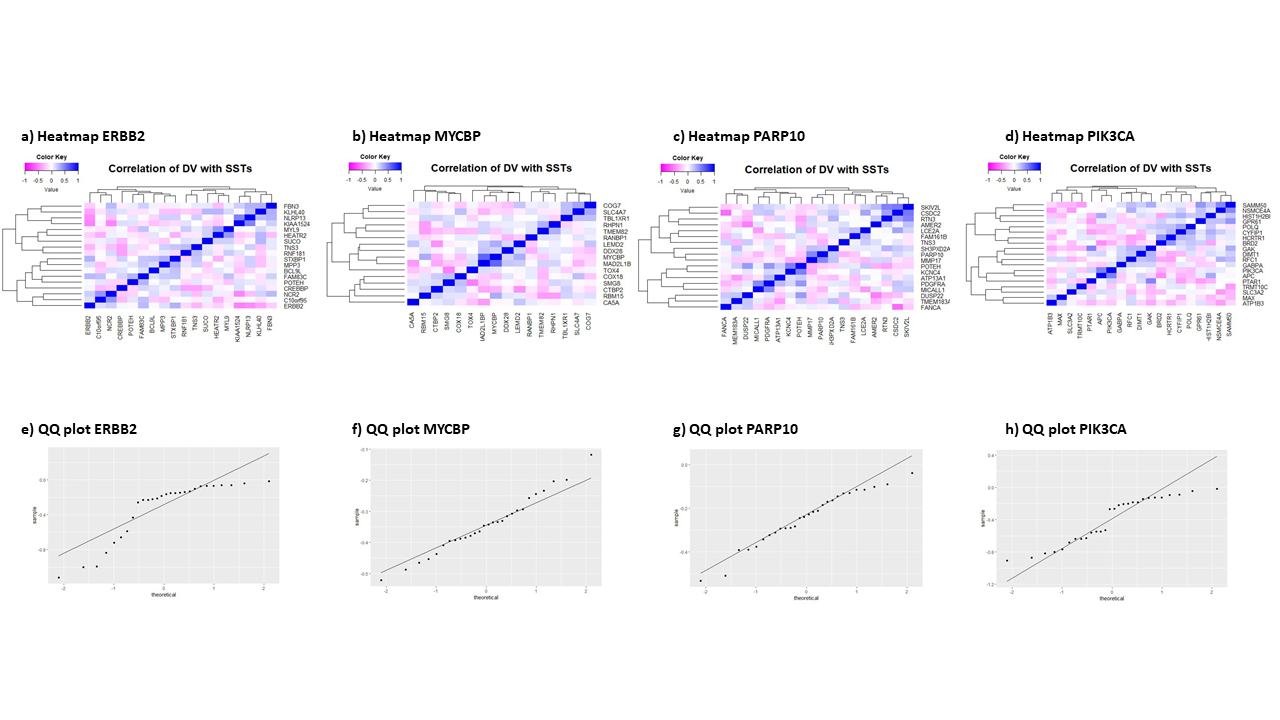
\includegraphics[width=1\linewidth]{File1}

\}

\textbackslash caption\{ \emph{Fig. 7} Heatmaps and QQ plots of
SSTs\}\label{fig:Hm and QQ} \textbackslash end\{figure\} The QQ-Plots
show that the sample Data of MYCBP and PARP10 is approx. normally
distributed while ERBB2 and PIK3CA do not show a normal distribution. As
one can see in the heatmaps of the Pearson correlation values, no
multicollinearity was detected, all x \textless{} 0.80.

\hypertarget{design-of-the-multilinear-regression}{%
\subsubsection{Design of the multilinear
regression}\label{design-of-the-multilinear-regression}}

To run the multilinear regression, it is advised to create a function
which splits the dataset in 75:25 (training set: testing set). Then the
function constructs a regression model with training data to predict DV
CERES (y; dep.variable) from SST CERES scores (x1 \ldots{} xn;
indep.variables) followed by checking model assumptions of residual
normal distribution and homoscedasticity. Later on, the function runs
the test data on model for performance evaluation and finally calculates
and plots the Spearman correlation to further asses model performance.

For the Spearman correlation, the rank-correlation coefficient can take
values from +1 to -1.

\begin{itemize}
\tightlist
\item
  rho \textasciitilde{} 1: perfect positive association of ranks
\item
  rho \textasciitilde{} 0: no association of ranks
\item
  rho \textasciitilde{} -1: perfect negative association of ranks
\end{itemize}

To further interpretate the p-value, we construct a H0 / H1 hypothesis:

\begin{itemize}
\tightlist
\item
  H0: There is no association between the predicted and observed
  variable.
\item
  H1: There is an association between the predicted and observed
  variable.
\end{itemize}

Most importantly, it is not possible to assess the strength of the
correlation based on the p-value. It rather judges the statistical test
than the resulting value. As default, we set the significance level to
0.05.

Subsequently, the latter values will be evaluated for the different
models. In case of a positive correlation, two variables move in the
same direction. For a well-designed model, we expect the predicted and
observed CERES scores to be approximately the same. Thus, optimal model
design is achieved if the correlation coefficient is close to 1 and the
p-value p \textless{} 0.05. Additionally, we plot the distributions of
predicted against observed values for each model.

\begin{Shaded}
\begin{Highlighting}[]
\NormalTok{input_data <-}\StringTok{ }\NormalTok{data_regression}

\NormalTok{plottingData <-}\StringTok{ }\KeywordTok{lapply}\NormalTok{(}\KeywordTok{seq_along}\NormalTok{(input_data), }\ControlFlowTok{function}\NormalTok{(a) \{}
  \KeywordTok{set.seed}\NormalTok{(}\DecValTok{123}\NormalTok{) }\CommentTok{#Initialize the random numbers, ensures better repoducibility}
\NormalTok{  data <-}\StringTok{ }\NormalTok{input_data[[a]] }\CommentTok{#Get the data}
  \KeywordTok{colnames}\NormalTok{(data)[}\KeywordTok{length}\NormalTok{(}\KeywordTok{colnames}\NormalTok{(data))] <-}\StringTok{ "Predictor"}
  
\NormalTok{  split =}\StringTok{ }\KeywordTok{sample.split}\NormalTok{(data[,}\KeywordTok{ncol}\NormalTok{(data)], }\DataTypeTok{SplitRatio =} \FloatTok{0.75}\NormalTok{) }\CommentTok{#Split the dataset into 3/4 Training and 1/4 Testing dataset}
\NormalTok{  training_set =}\StringTok{ }\KeywordTok{subset}\NormalTok{(data, split }\OperatorTok{==}\StringTok{ }\OtherTok{TRUE}\NormalTok{) }\CommentTok{#Use the labels to get the training data}
\NormalTok{  test_set =}\StringTok{ }\KeywordTok{subset}\NormalTok{(data, split }\OperatorTok{==}\StringTok{ }\OtherTok{FALSE}\NormalTok{)}
  
\NormalTok{  regressor =}\StringTok{ }\KeywordTok{lm}\NormalTok{(}\DataTypeTok{formula =}\NormalTok{ Predictor }\OperatorTok{~}\StringTok{ }\NormalTok{., }
                 \DataTypeTok{data =}\NormalTok{ training_set)  }\CommentTok{#Predict CERES of Driver Mutation based on all (=.) the input variables (SSTs)}
  
  \KeywordTok{pdf}\NormalTok{(}\KeywordTok{paste0}\NormalTok{(root.dir, }\StringTok{"/Resid-HomoPlot_"}\NormalTok{,drivermut[a],}\StringTok{".pdf"}\NormalTok{)) }\CommentTok{#Save plots as pdf, in root directory}
  \KeywordTok{hist}\NormalTok{(}\KeywordTok{resid}\NormalTok{(regressor), }\DataTypeTok{main =} \KeywordTok{paste0}\NormalTok{(}\StringTok{'Histogram of residuals: '}\NormalTok{, driver_mut[a]),}\DataTypeTok{xlab=}\StringTok{'Standardised Residuals'}\NormalTok{,}\DataTypeTok{ylab=}\StringTok{'Frequency'}\NormalTok{) }\CommentTok{#Plot a histogram of standardised residuals to check the assumption of normality}
  \KeywordTok{dev.off}\NormalTok{() }\CommentTok{#Closing the figure file}
  
  \KeywordTok{pdf}\NormalTok{(}\KeywordTok{paste0}\NormalTok{(root.dir, }\StringTok{"/HomoPlot_"}\NormalTok{,drivermut[a],}\StringTok{".pdf"}\NormalTok{)) }\CommentTok{#Save plots as pdf, in working directory "wd"}
  \KeywordTok{plot}\NormalTok{(regressor, }\DataTypeTok{which =} \DecValTok{1}\NormalTok{) }\CommentTok{#Fitted values and residuals plot to check the assumption of homoscedasticity}
  \KeywordTok{dev.off}\NormalTok{() }\CommentTok{#Closing the figure file}
  
\NormalTok{  y_pred =}\StringTok{ }\KeywordTok{predict}\NormalTok{(regressor, }\DataTypeTok{newdata =}\NormalTok{ test_set) }\CommentTok{#Predict the Driver mut. CERES score based on the test data}
\NormalTok{  test_set}\OperatorTok{$}\NormalTok{Prediction =}\StringTok{ }\NormalTok{y_pred }\CommentTok{#Adding predictions to the dataset}
  
\NormalTok{  df =}\StringTok{ }\KeywordTok{cbind}\NormalTok{(test_set}\OperatorTok{$}\NormalTok{Predictor, test_set}\OperatorTok{$}\NormalTok{Prediction)}
  \KeywordTok{colnames}\NormalTok{(df) <-}\StringTok{ }\KeywordTok{c}\NormalTok{(}\StringTok{"Predictor"}\NormalTok{, }\StringTok{"Prediction"}\NormalTok{)}
  \KeywordTok{rownames}\NormalTok{(df) <-}\StringTok{ }\KeywordTok{rownames}\NormalTok{(test_set)}
  
  \KeywordTok{return}\NormalTok{(df) }\CommentTok{#Create a dataframe with predicted and observed CERES values}
\NormalTok{\})}

\CommentTok{#Plot the data external }
\NormalTok{plottingFunction <-}\StringTok{ }\ControlFlowTok{function}\NormalTok{(inputData, driverMut) \{ }\CommentTok{#Design plot function observed vs. predicted values}
\NormalTok{  df =}\StringTok{ }\KeywordTok{melt}\NormalTok{(inputData) }\CommentTok{#Default for ggplot}
\NormalTok{  p <-}\StringTok{ }\KeywordTok{ggplot}\NormalTok{(}\DataTypeTok{data =}\NormalTok{ df, }\KeywordTok{aes}\NormalTok{(}\DataTypeTok{x=}\NormalTok{value, }\DataTypeTok{fill=}\NormalTok{Var2)) }\OperatorTok{+}\StringTok{ }
\StringTok{    }\KeywordTok{geom_density}\NormalTok{(}\DataTypeTok{alpha=}\NormalTok{.}\DecValTok{3}\NormalTok{) }\OperatorTok{+}
\StringTok{    }\KeywordTok{ggtitle}\NormalTok{(}\KeywordTok{paste0}\NormalTok{(}\StringTok{"Spearman Correlation plot: "}\NormalTok{, driverMut)) }\OperatorTok{+}
\StringTok{    }\KeywordTok{ylab}\NormalTok{(}\StringTok{"Predicted score"}\NormalTok{) }\OperatorTok{+}
\StringTok{    }\KeywordTok{xlab}\NormalTok{(}\StringTok{"Observed score"}\NormalTok{) }\OperatorTok{+}
\StringTok{    }\KeywordTok{theme_bw}\NormalTok{(}\DataTypeTok{base_size =} \DecValTok{7}\NormalTok{) }\OperatorTok{+}\StringTok{ }\CommentTok{#Design input}
\StringTok{    }\KeywordTok{theme}\NormalTok{(}\DataTypeTok{legend.position=}\StringTok{"bottom"}\NormalTok{,}
          \DataTypeTok{legend.direction=}\StringTok{"horizontal"}\NormalTok{,}
          \DataTypeTok{plot.title =} \KeywordTok{element_text}\NormalTok{(}\DataTypeTok{hjust =} \FloatTok{0.5}\NormalTok{),}
          \DataTypeTok{axis.text.x =} \KeywordTok{element_text}\NormalTok{(}\DataTypeTok{angle =} \DecValTok{90}\NormalTok{, }\DataTypeTok{vjust =} \FloatTok{0.5}\NormalTok{, }\DataTypeTok{hjust=}\DecValTok{1}\NormalTok{),}\CommentTok{#Design input}
          \DataTypeTok{legend.title=} \KeywordTok{element_blank}\NormalTok{(),}
          \DataTypeTok{axis.title.x =} \KeywordTok{element_blank}\NormalTok{(),}
          \DataTypeTok{strip.text.y =} \KeywordTok{element_text}\NormalTok{(}\DataTypeTok{angle =} \DecValTok{0}\NormalTok{))}
  
  \KeywordTok{pdf}\NormalTok{(}\KeywordTok{paste0}\NormalTok{(root.dir, }\StringTok{"/SpearmanPlot"}\NormalTok{,driverMut,}\StringTok{".pdf"}\NormalTok{)) }\CommentTok{#Save plots as pdf, in root directory}
  \KeywordTok{print}\NormalTok{(p)}
  \KeywordTok{dev.off}\NormalTok{()}\CommentTok{#Closing the figure file}
\NormalTok{\}}

\KeywordTok{plottingFunction}\NormalTok{(plottingData[[}\DecValTok{1}\NormalTok{]], drivermut[}\DecValTok{1}\NormalTok{])}
\end{Highlighting}
\end{Shaded}

\begin{verbatim}
## pdf 
##   2
\end{verbatim}

\begin{Shaded}
\begin{Highlighting}[]
\KeywordTok{plottingFunction}\NormalTok{(plottingData[[}\DecValTok{2}\NormalTok{]], drivermut[}\DecValTok{2}\NormalTok{])}
\end{Highlighting}
\end{Shaded}

\begin{verbatim}
## pdf 
##   2
\end{verbatim}

\begin{Shaded}
\begin{Highlighting}[]
\KeywordTok{plottingFunction}\NormalTok{(plottingData[[}\DecValTok{3}\NormalTok{]], drivermut[}\DecValTok{3}\NormalTok{])}
\end{Highlighting}
\end{Shaded}

\begin{verbatim}
## pdf 
##   2
\end{verbatim}

\begin{Shaded}
\begin{Highlighting}[]
\KeywordTok{plottingFunction}\NormalTok{(plottingData[[}\DecValTok{4}\NormalTok{]], drivermut[}\DecValTok{4}\NormalTok{])}
\end{Highlighting}
\end{Shaded}

\begin{verbatim}
## pdf 
##   2
\end{verbatim}

\begin{Shaded}
\begin{Highlighting}[]
\CommentTok{#Get the correlation values}
\NormalTok{correlations <-}\StringTok{ }\KeywordTok{lapply}\NormalTok{(}\KeywordTok{seq_along}\NormalTok{(plottingData), }\ControlFlowTok{function}\NormalTok{(a) \{}
\NormalTok{  df =}\StringTok{ }\NormalTok{plottingData[[a]]}
\NormalTok{  corVal <-}\StringTok{ }\KeywordTok{cor.test}\NormalTok{(df[,}\DecValTok{1}\NormalTok{] , df[,}\DecValTok{2}\NormalTok{], }\DataTypeTok{method =} \StringTok{"spearman"}\NormalTok{) }\CommentTok{#To judge model performance, calculate Spearman corr. between predicted and observed values}
  \KeywordTok{return}\NormalTok{(corVal)}
\NormalTok{\})}
\KeywordTok{names}\NormalTok{(correlations) <-}\StringTok{ }\NormalTok{drivermut}
\NormalTok{correlations }\CommentTok{#Look at the data}
\end{Highlighting}
\end{Shaded}

\begin{verbatim}
## $ERBB2
## 
##  Spearman's rank correlation rho
## 
## data:  df[, 1] and df[, 2]
## S = 50, p-value = 0.8397
## alternative hypothesis: true rho is not equal to 0
## sample estimates:
##       rho 
## 0.1071429 
## 
## 
## $MYCBP
## 
##  Spearman's rank correlation rho
## 
## data:  df[, 1] and df[, 2]
## S = 64, p-value = 0.7825
## alternative hypothesis: true rho is not equal to 0
## sample estimates:
##        rho 
## -0.1428571 
## 
## 
## $PARP10
## 
##  Spearman's rank correlation rho
## 
## data:  df[, 1] and df[, 2]
## S = 94, p-value = 0.1095
## alternative hypothesis: true rho is not equal to 0
## sample estimates:
##        rho 
## -0.6785714 
## 
## 
## $PIK3CA
## 
##  Spearman's rank correlation rho
## 
## data:  df[, 1] and df[, 2]
## S = 66, p-value = 0.7131
## alternative hypothesis: true rho is not equal to 0
## sample estimates:
##        rho 
## -0.1785714
\end{verbatim}

All four models were tested on the assumptions. The following table
provides a quick overview of whether constructed assumptions were met
(yes) or not (no). For multicollinarity, all models met the condition r
\textless{} 0.8 for all variables.

\begin{longtable}[]{@{}lllll@{}}
\toprule
\begin{minipage}[b]{0.10\columnwidth}\raggedright
Model\strut
\end{minipage} & \begin{minipage}[b]{0.19\columnwidth}\raggedright
Data distribution\strut
\end{minipage} & \begin{minipage}[b]{0.21\columnwidth}\raggedright
Residual distribution\strut
\end{minipage} & \begin{minipage}[b]{0.16\columnwidth}\raggedright
Homoscedastity\strut
\end{minipage} & \begin{minipage}[b]{0.20\columnwidth}\raggedright
Spearman correlation\strut
\end{minipage}\tabularnewline
\midrule
\endhead
\begin{minipage}[t]{0.10\columnwidth}\raggedright
ERBB2\strut
\end{minipage} & \begin{minipage}[t]{0.19\columnwidth}\raggedright
no\strut
\end{minipage} & \begin{minipage}[t]{0.21\columnwidth}\raggedright
yes\strut
\end{minipage} & \begin{minipage}[t]{0.16\columnwidth}\raggedright
no\strut
\end{minipage} & \begin{minipage}[t]{0.20\columnwidth}\raggedright
no\strut
\end{minipage}\tabularnewline
\begin{minipage}[t]{0.10\columnwidth}\raggedright
MCYBP\strut
\end{minipage} & \begin{minipage}[t]{0.19\columnwidth}\raggedright
yes\strut
\end{minipage} & \begin{minipage}[t]{0.21\columnwidth}\raggedright
no\strut
\end{minipage} & \begin{minipage}[t]{0.16\columnwidth}\raggedright
yes\strut
\end{minipage} & \begin{minipage}[t]{0.20\columnwidth}\raggedright
no\strut
\end{minipage}\tabularnewline
\begin{minipage}[t]{0.10\columnwidth}\raggedright
PARP10\strut
\end{minipage} & \begin{minipage}[t]{0.19\columnwidth}\raggedright
yes\strut
\end{minipage} & \begin{minipage}[t]{0.21\columnwidth}\raggedright
no\strut
\end{minipage} & \begin{minipage}[t]{0.16\columnwidth}\raggedright
yes\strut
\end{minipage} & \begin{minipage}[t]{0.20\columnwidth}\raggedright
no\strut
\end{minipage}\tabularnewline
\begin{minipage}[t]{0.10\columnwidth}\raggedright
PIK3CA\strut
\end{minipage} & \begin{minipage}[t]{0.19\columnwidth}\raggedright
no\strut
\end{minipage} & \begin{minipage}[t]{0.21\columnwidth}\raggedright
yes\strut
\end{minipage} & \begin{minipage}[t]{0.16\columnwidth}\raggedright
no\strut
\end{minipage} & \begin{minipage}[t]{0.20\columnwidth}\raggedright
no\strut
\end{minipage}\tabularnewline
\bottomrule
\end{longtable}

Checking distributional assumptions (= normal distribution) is also
important and a different model should be chosen if needed (Harrell,
2001). As shown in the qq-Plots, normal distribution does only apply to
the models of MYCBP and PARP10. ERBB2 on the other hand, delivers the
highest rho, but is in not approximately normally distributed. The
PIK3CA model also does not fulfill the condition of being normally
distributed.

The normal distribution does not lead to higher correlation
coefficients. Unmet distribution assumptions should be treated as a red
flag suggesting this model not to be suited for further use.

Residual are the differences between actual and predicted y-values . For
a good model, we expect the model to return positive and negative
residual values with the same chance, resulting in residual normal
distribution (Motulsky 2018). The residual distribution of ERBB2 was
closest to normal distribution. The PIK3CA residuals showed still
acceptable approximation of normal distribution. MYCBP and PARP10 failed
to show approximate normal residual distribution.

Homoscedastity is also known as homogeneity of variance, assuming that
the probability distribution for the response variable has the same
standard deviation, independent of the x value.This condition is met if
random variables have similar variance. Also, there is no pattern of
variance change if the random variables in- or decrease. (Achen and
Shively 1995)

ERBB2 and PIK3CA violate the condition, while MYCBP and PARP10 show
homoscedasticity.

We obtained the following p-values and correlation coefficients:

\begin{longtable}[]{@{}lllll@{}}
\toprule
Model & p-value & accepted hypothesis & rho & relationship
type\tabularnewline
\midrule
\endhead
ERBB2 & 0.8397 & H0 & 0.1071 & weak positive\tabularnewline
MCYBP & 0.7825 & H0 & -0.1429 & weak negative\tabularnewline
PARP10 & 0.1095 & H0 & -0.6786 & moderate negative\tabularnewline
PIK3CA & 0.7131 & H0 & -0.1786 & weak negative\tabularnewline
\bottomrule
\end{longtable}

The ERBB2-model shows the highest rho value of all four models, but
\textasciitilde{} 0.1 is a rather weak positive relationship.The p-value
leads to acceptance of H0.

The rho value of the MYCBP-model leads to very weak negative
correlation. A p-value of \textasciitilde{} 0.78 leads to confident
acceptance of H0.

For the PARP10-model, the rho value of \textasciitilde{} -0.68 is a
moderate negative relationship. The p-value leads to acceptance of H0
and is lowest with \textasciitilde{} 0.11. But even if we would raise
the confidence level to 0.10 (which would be questionable in
statistics), the result wouldn?t be significant to accept H1.

The rho value of the PIK3CA-model leads to very weak negative
correlation. A p-value of \textasciitilde{} 0.78 leads to confident
acceptance of H0.

The models for MYCBP and PIK3CA only showed weak, negative correlation,
which is not useful for further work with this model. The PARP10 model
resulted in a moderate negative relationship, which is not of relevance
for our objective. The ERBB2 model did not deliver a significant
p-value, but indeed contains at least a weak positive correlation.

\hypertarget{discussion-of-the-regression-model}{%
\subsection{Discussion of the regression
model}\label{discussion-of-the-regression-model}}

All in all, all multilinear regression models failed to meet all
regression prerequisites and do not deliver a p-value of significant
relevance for the correlation. Thus, they should not be used for further
predictions. Especially the models for ERBB2 and PIK3CA should have been
discarded, since the sample values are not even normally distributed. It
seems possible that the small sample size for the regression model lead
to the lack of significant results, with only 28 events (CERES score
observed in cell line) per predicting variable (SST gene).

But, a common rule for building a regression model is to calculate the
\emph{limiting sample size}: In summary it can thus be argued that these
multilinear regression models are not effective in predicting the impact
of DVs on cell viability. One possible reason for unfitting regression
models could be the small sample size of only 28 events (breast cancer
cell lines). A rule of thumb for building a regression model is to
calculate the limiting sample size:

\(p < \frac{m}{15}\)

\begin{itemize}
\tightlist
\item
  p: number of predictor variables
\item
  m: limiting sample size; for continuous response variables it is the
  total sample size n
\end{itemize}

If this equation is fulfilled, the model is supposed to be
reliable.(Harrell, 2001) In fact, this condition is true for all four
models.

Our data seems to have an appropriate size for a basic regression model.
On the other hand, for the supervised machine learning process of the
regression, sample sizes up to n = 50,000 are reported. (Libbrecht and
Noble, 2015) In general, more data will lead to improved regression
quality. Generally, scientists are advised to focus on obtaining and
analyzing larger data sets instead of comparing different learning
techniques on small training sets. (Banko and Brill, 2001)

\hypertarget{results-and-discussion}{%
\section{Results and Discussion}\label{results-and-discussion}}

The aim of this project was to identify genes, so called second-site
targets (SSTs), which interact genetically with selected driver
mutations (DVs) to promote cell viability and proliferation in breast
cell cancers. Our hope is that these genes could be potential new
targets for more specific therapies.

After selection of five non-tumor suppressor gene DVs (CCND, ERBB2, MYC,
PARP10, PIK3CA) from literature datasets were formatted to include only
breast cancer cell lines. Subsequent, general data exploration revealed
a large variety of CERES scores and expression values across both
selected DVS and remaining genes of breast cell cancer lines. This
proved the need to undertake further steps of data cleanup. Thus, in
order to analyze only mutated genes, the \texttt{mutImpact} matrix was
generated, containing CERES values only of mutated genes in a given cell
line, otherwise with the entry for a given cell line being \texttt{NA}.
Further cleanup was performed by removing all genes which displaying
only \texttt{NA} values and whose mean CERES scores were greater than
zero. Through this process, 4934 possible SST genes remained, fitting
the criteria of being mutated and having a positive impact on cell
viability. However, in this process genes with a nonuniform distribution
or of CERES scores across cell lines or unique outliers distorting mean
values could have been mistakenly removed.

With these findings, the selection of DVs from literature research was
verified by performing k means clustering of associated CERES scores.
After calculation of within sum squares values for a range of cluster
numbers, the optimal cluster number was identified to be four, using the
elbow method. Clustering revealed four out of five driver mutations to
be colocalized in cluster three, hence, simlarly improving the viability
of breast cancer cells while not being tumor suppressor genes. These
genes thus proved appropriate for further analysis. While CCND was
removed early on in data clean up stages due to not being mutated in any
breast cancer cell line, ERBB2IP was found in cluster four and, thus,
excluded from further analysis. Overall, it must be noted that although
the optimal cluster number was identified to be four, the cluster plot
shows that clusters were not distinctly separated from one another.
Alternative cluster numbers could therefore have resulted in a different
assignment of DVs and consequently other results based on our selection
method.

Nevertheless ERBB2, MYCBP, PARP10 and PIK3CA were used as central DVs
for further analysis. Box and whisker plots of CERES scores revealed
mutations of the MYCB gene to have greatest essentiality, with least
variation, for cell survival. ERBB2 on the other hand had the highest
average of CERES scores, greatest variation and lowest impact on cell
proliferation. In contrast the ERBB2 DV showed highest TPM values and
hence suggested overexpression. However, it remained the gene with
greatest variation in values closely followed by PARP10. TPM expression
values were lowest for PIK3CA, with little variation which was also seen
for MYCBP.

As SSTs are genes expected to interact synergistically with the
corresponding driver mutation in promoting cell viability, CERES values
were expected to be similar to those of the corresponding DVs.
Consequently, all 1171 genes colocalized in k means cluster 3 were
regarded as potential SST candidates. In order to spot genetic
interactions, the paired statistical Wilcoxon test was performed, given
that data followed a non-normal distribution. SST candiates were chosen
by the means of the highest p-values serving as a measure of similarity
of CERES scores and, thus, genetic interaction. Surprisingly, the first
quantile was set at a p-value of 0.0 for each driver mutation,
indicating that many genes had CERES score not relatable to the CERES
cores of driver mutations. The maximum p-value of each test however
constituted 1.0, suggesting that there were also genes with similar
CERES scores to driver mutations.

Based on the result of the Wilcoxon test, the top 15 genes with highest
p-values for each mutation were chosen. Due to some genes having the
same p-value, ERBB2 and PARP10 were each found to have 17 potential SST
candidates, PIK3CA 18 potential candidates while MYCBP had 15
candidates. In the next step all potential SST candidates were verified,
by checking their cluster assignment in the previously completed k means
clustering. As expected, all SST candidates were confirmed to be found
in in the same cluster 3 as the DVs. With this verification, all SSTs
were characterized and labelled with mutation type and the physiological
gene function using the universal protein database (UniProt). The most
common type of mutation was a missense or silent mutation for SSTs of
all driver mutations. Most strikingly, many SST gene functions comprised
proteins contributing to cell cycle progression, cell motility and
polarity together with transcriptional regulators affecting cell
metabolism.

After discovering all functions of the SSTs candidates we investigated
if research exploring their therapeutic potential has already been
published. In our cohort of 67 SSTs only one SST is already targetable
with a drug. While a few of them are hardly present in ongoing research,
most of the SSTs have be already been related to tumor diseases. Upon
further investigation the four SSTs TNS3, BCL9L, CREBBP and SLC4A7
represent the main targets for future therapy investigations. We would
be thrilled to see some of them in a drug database in the future.

The final step in this project, was to exploit the identified
interactions and design a regression model to predict CERES scores of
DVs based on the SST candidate CERES scores. This would allow us to
predict the impact of driver mutations on cell viability based on the
effect of SSTs on breast cancer cell proliferation. After data
preparation, the conditions of normality and multicollinearity were
verified. While MYCBP and PARP10 CERES values were approximately
normally distributed, ERBB2 and PIK3CA values were not, thus not meeting
the criteria for a multilinear regression. Additionally, no
multicollinearity was detected with all rho values smaller than 0.80.

\begin{longtable}[]{@{}lllll@{}}
\toprule
\begin{minipage}[b]{0.10\columnwidth}\raggedright
Model\strut
\end{minipage} & \begin{minipage}[b]{0.19\columnwidth}\raggedright
Data distribution\strut
\end{minipage} & \begin{minipage}[b]{0.21\columnwidth}\raggedright
Residual distribution\strut
\end{minipage} & \begin{minipage}[b]{0.16\columnwidth}\raggedright
Homoscedastity\strut
\end{minipage} & \begin{minipage}[b]{0.20\columnwidth}\raggedright
Spearman correlation\strut
\end{minipage}\tabularnewline
\midrule
\endhead
\begin{minipage}[t]{0.10\columnwidth}\raggedright
ERBB2\strut
\end{minipage} & \begin{minipage}[t]{0.19\columnwidth}\raggedright
no\strut
\end{minipage} & \begin{minipage}[t]{0.21\columnwidth}\raggedright
yes\strut
\end{minipage} & \begin{minipage}[t]{0.16\columnwidth}\raggedright
no\strut
\end{minipage} & \begin{minipage}[t]{0.20\columnwidth}\raggedright
no\strut
\end{minipage}\tabularnewline
\begin{minipage}[t]{0.10\columnwidth}\raggedright
MCYBP\strut
\end{minipage} & \begin{minipage}[t]{0.19\columnwidth}\raggedright
yes\strut
\end{minipage} & \begin{minipage}[t]{0.21\columnwidth}\raggedright
no\strut
\end{minipage} & \begin{minipage}[t]{0.16\columnwidth}\raggedright
yes\strut
\end{minipage} & \begin{minipage}[t]{0.20\columnwidth}\raggedright
no\strut
\end{minipage}\tabularnewline
\begin{minipage}[t]{0.10\columnwidth}\raggedright
PARP\strut
\end{minipage} & \begin{minipage}[t]{0.19\columnwidth}\raggedright
yes\strut
\end{minipage} & \begin{minipage}[t]{0.21\columnwidth}\raggedright
no\strut
\end{minipage} & \begin{minipage}[t]{0.16\columnwidth}\raggedright
yes\strut
\end{minipage} & \begin{minipage}[t]{0.20\columnwidth}\raggedright
no\strut
\end{minipage}\tabularnewline
\begin{minipage}[t]{0.10\columnwidth}\raggedright
PIK3CA\strut
\end{minipage} & \begin{minipage}[t]{0.19\columnwidth}\raggedright
no\strut
\end{minipage} & \begin{minipage}[t]{0.21\columnwidth}\raggedright
yes\strut
\end{minipage} & \begin{minipage}[t]{0.16\columnwidth}\raggedright
no\strut
\end{minipage} & \begin{minipage}[t]{0.20\columnwidth}\raggedright
no\strut
\end{minipage}\tabularnewline
\bottomrule
\end{longtable}

\begin{verbatim}
## [1] "Table  1: Summary of the Regression assumption checks for the four models. Conditions were met (yes) or not (no)."
\end{verbatim}

Nevertheless, after training the model on 75\% of the data, the
multilinear regression was run and residual normal distribution and
homoscedasticity as requirements for a good model, were analyzed. While
the residuals of ERBB2 were closest to a normal distribution, residuals
of the PIK3CA model are still an acceptable approximate of a normal
distribution. On the other hand MYCBP and PARP10 do not show a normal
residual distribution while they do meet the condition of
homoscedasticity, unlike ERBB2 and PIK3CA. A further measure to evaluate
the design of the model was the test of Spearman correlation. P-values
of all DVs lead to the confident acceptance of the H0 hypothesis and
hence the statement that there is no association between predicted and
observed variable. Weak negative correlation was identified for the
MYCBP and PIK3CA model compared to a moderate negative correlation for
the PARP10-model. Surprisingly, the ERBB2-model with a rho-value of 0.1
shows a weak positive relationship.

\begin{longtable}[]{@{}lllll@{}}
\toprule
Model & p-value & accepted hypothesis & rho & relationship
type\tabularnewline
\midrule
\endhead
ERBB2 & 0.8397 & H0 & 0.1071 & weak positive\tabularnewline
MCYBP & 0.7825 & H0 & -0.1429 & weak negative\tabularnewline
PARP10 & 0.1095 & H0 & -0.6786 & moderate negative\tabularnewline
PIK3CA & 0.7131 & H0 & -0.1786 & weak negative\tabularnewline
\bottomrule
\end{longtable}

\begin{verbatim}
## [1] "Table  2: Summary of Spearman Correlation Test between observed and predicted values. Including p-value and the thus accepted hypothesis, as well as the correlation value rho and the corresponding strenght of the linear relationship."
\end{verbatim}

To improve the quality of the model, especially for the unsupervised
machine learning process, a larger dataset might be necessary for the
construction of an appropriate model and leads in general to improved
results. It might be helpful to obtain and analyze larger data sets
instead of comparing different learning techniques on small training
sets (Banko and Brill, 2001). For expample, sample sizes up to n =
50,000 are reported for comparable tasks (Libbrecht and Noble, 2015). It
should also be considered, that CERES scores of SST candidates and DVs
may have a nonlinear correlation, requiring different prediction models.

\hypertarget{literature}{%
\section{Literature}\label{literature}}

\begin{itemize}
\tightlist
\item
  Achen, C. H. and W. P. Shively (1995). Cross-Level Inference,
  University of Chicago Press.
\item
  Aleskandarany, M. A., E. A. Rakha, M. A. H. Ahmed, D. G. Powe, E. C.
  Paish, R. D. Macmillan, I. O. Ellis and A. R. Green (2010). ``PIK3CA
  expression in invasive breast cancer: a biomarker of poor prognosis.''
  Breast Cancer Research and Treatment 122(1): 45-53.
\item
  Anderson, M. W., Reynolds, S. H., You, M., \& Maronpot, R. M. (1992).
  Role of proto-oncogene activation in carcinogenesis. Environmental
  health perspectives, 98, 13-24.
\item
  Arnold, A. and A. Papanikolaou (2005). ``Cyclin D1 in Breast Cancer
  Pathogenesis.'' Journal of Clinical Oncology 23(18): 4215-4224.
\item
  Ashworth, A., Lord, Christopher?J., \& Reis-Filho, Jorge?S. (2011).
  Genetic Interactions in Cancer Progression and Treatment. Cell,
  145(1), 30-38.
\item
  Barnes, B., K. Kraywinkel, E. Nowossadeck, I. Schönfeld, A.
  Starker, A. Wienecke and U. Wolf (2016). Bericht zum Krebsgeschehen in
  Deutschland 2016, Robert Koch-Institut.
\item
  Banko, M. and E. Brill (2001). Scaling to very very large corpora for
  natural language disambiguation. Proceedings of the 39th Annual
  Meeting on Association for Computational Linguistics. Toulouse,
  France, Association for Computational Linguistics: 26-33.
\item
  Benstead-Hume, G., Wooller Sarah, K., \& Pearl Frances, M. G. (2017).
  Computational Approaches to Identify Genetic Interactions for Cancer
  Therapeutics. In Journal of Integrative Bioinformatics (Vol. 14).
\item
  Gabay, M., Y. Li and D. W. Felsher ``MYC activation is a hallmark of
  cancer initiation and maintenance.'' Cold Spring Harbor perspectives
  in medicine 4(6): a014241.
\item
  Hanahan, D., \& Weinberg, R. A. (2000). The hallmarks of cancer. Cell,
  100(1), 57-70.
\item
  Harrell, F. E. (2001). Regression modeling strategies : with
  applications to linear models, logistic regression, and survival
  analysis. New York ; Berlin ; Heidelberg {[}u.a.{]}, Springer.
\item
  Hutchinson, L. (2010). ``Challenges, controversies, breakthroughs.''
  Nature Reviews Clinical Oncology 7: 669.
\item
  Koch-Institut, R. (2017). Krebs in Deutschland für 2013/2014,
  Robert Koch-Institut.
\item
  Kumar R (2016) A novel therapeutic target for triple negative breast
  cancer. Biomed Genet Genomics. 1: DOI: 10.15761/BGG.1000101.
\item
  Lacouture, M., \& Sibaud, V. (2018). Toxic Side Effects of Targeted
  Therapies and Immunotherapies Affecting the Skin, Oral Mucosa, Hair,
  and Nails. Am J Clin Dermatol, 19(Suppl 1), 31-39.
\item
  Lee, E. Y. H. P., \& Muller, W. J. (2010). Oncogenes and tumor
  suppressor genes. Cold Spring Harbor perspectives in biology, 2(10),
  a003236-a003236.
\item
  Libbrecht, M. W. and W. S. Noble (2015). ``Machine learning
  applications in genetics and genomics.'' Nature reviews. Genetics
  16(6): 321-332.
\item
  Magen, A., Das, A., Sang Lee, J., Sharmin, M., Lugo, A., Gutkind, S.,
  . . . Hannenhalli, S. (2018). Beyond synthetic lethality: multiple
  gene interaction types play a key functional role in cancer. bioRxiv,
  25312.
\item
  Maximiano, S., Magalhaes, P., Guerreiro, M. P., \& Morgado, M. (2016).
  Trastuzumab in the Treatment of Breast Cancer. BioDrugs, 30(2), 75-86.
\item
  Motulsky, H. (2018). Intuitive biostatistics : a nonmathematical guide
  to statistical thinking. New York ; London, Oxford University Press.
\item
  Nussinov, R., Jang, H., Tsai, C.-J., \& Cheng, F. (2019). Review:
  Precision medicine and driver mutations: Computational methods,
  functional assays and conformational principles for interpreting
  cancer drivers. PLoS computational biology, 15(3), e1006658-e1006658.
\item
  Rauscher, B., Heigwer, F., Henkel, L., Hielscher, T., Voloshanenko,
  O., \& Boutros, M. (2018). Toward an integrated map of genetic
  interactions in cancer cells. Molecular systems biology, 14(2),
  e7656-e7656.
\item
  Seimiya, H. (2015). {[}Cancer therapy by PARP inhibitors{]}. Nihon
  Rinsho, 73(8), 1330-1335.
\item
  Shimoi, T., A. Hamada, M. Yamagishi, M. Hirai, M. Yoshida, T.
  Nishikawa, K. Sudo, A. Shimomura, E. Noguchi, M. Yunokawa, K.
  Yonemori, C. Shimizu, T. + Kinoshita, T. Fukuda, Y. Fujiwara and K.
  Tamura (2018). ``PIK3CA mutation profiling in patients with breast
  cancer, using a highly sensitive detection system.'' Cancer science
  109(8): 2558-2566.
\item
  Siraj, A. K., P. Pratheeshkumar, S. K. Parvathareddy, S. P. Divya, F.
  Al-Dayel, A. Tulbah, D. Ajarim and K. S. Al-Kuraya (2018).
  ``Overexpression of PARP is an independent prognostic marker for poor
  survival in Middle Eastern breast cancer and its inhibition can be
  enhanced with embelin co-treatment.'' Oncotarget 9(99): 37319-37332.
\item
  Slamon, D., W. Godolphin, L. Jones, J. Holt, S. Wong, D. Keith, W.
  Levin, S. Stuart, J. Udove, A. Ullrich and a. et (1989). ``Studies of
  the HER-2/neu proto-oncogene in human breast and ovarian cancer.''
  Science 244(4905): 707-712.
\item
  Sledge, G.W. u. a., 2014. Past, present, and future challenges in
  breast cancer treatment. Journal of clinical oncology???: official
  journal of the American Society of Clinical Oncology, 32(19),
  S.1979-1986.
\item
  Stratton, M. R., P. J. Campbell and P. A. Futreal (2009). ``The cancer
  genome.'' Nature 458(7239): 719-724.
\item
  Tsilimigras, D. I., Ntanasis-Stathopoulos, I., Bagante, F., Moris, D.,
  Cloyd, J., Spartalis, E., \& Pawlik, T. M. (2018). Clinical
  significance and prognostic relevance of KRAS, BRAF, PI3K and TP53
  genetic mutation analysis for resectable and unresectable colorectal
  liver metastases: A systematic review of the current evidence. Surg
  Oncol, 27(2), 280-288.
\item
  Xu, J., Y. Chen and O. I. Olopade (2010). ``MYC and Breast Cancer.''
  Genes \& cancer 1(6): 629-640.
\end{itemize}


\end{document}
